\documentclass[bg]{copernicus}
\usepackage[T1]{fontenc}
\usepackage[latin1]{inputenc}
\usepackage{natbib}
\usepackage{color}
\bibliographystyle{copernicus}

\newcommand{\pa}[1]{{\Large PA: #1}}

\newcommand{\nx}[1]{N_{\mbox{\tiny\textsc{#1}}}}
\newcommand{\nsom}{\nx{som}}
\newcommand{\nsmb}{\nx{smb}}
\newcommand{\naom}{\nx{aom}}

\begin{document}

\title{Initializing organic matter pools}
\author{P. Abrahamsen}
\author{B. Gjettermann}
\author{S. Hansen}
\affil{University of Copenhagen, Faculty of Life Sciences,\\
  Department of Basic Sciences and Environment, Agrohydrology. \\
  Torvaldsensvej 40, DK-1871 Frederiksberg, Denmark.}

\runningtitle{Initializing organic matter pools}
\runningauthor{P.~Abrahamsen et al.}
\correspondence{P.~Abrahamsen (pa@life.ku.dk)}

\maketitle

\begin{abstract}
  Organic matter models using multiple pools for soil microbial
  biomass and soil organic matter have proved able to simulate both
  short term and long term change in humus content of agricultural
  soil. However, these pools do not correspond to measurable physical
  quantities, and are therefore difficult for a non-expert to
  understand and use. To initialize these pools it is often assumed
  that organic matter is in a state of equilibrium. Unfortunately, the
  time to reach equilibrium is often measured in centuries. Therefore
  the use of a warm-up period cannot replace the need for a good
  initial partitioning. In this paper we examine a weaker assumption,
  namely a quasi-equilibrium where all except for the slowest pool is
  in equilibrium with the amount of carbon input. This assumption
  allows the non-expert user to initialize the model, and is robust
  with regard to model changes.  We compare the initialization
  resulting from the equilibrium and the quasi-equilibrium with long
  term dynamic simulations, and discuss where each method is most
  applicable.
\end{abstract}

\introduction

Weather-driven simulation modeling has become an important component
of studies of soil nutrients and carbon balances in relation to soil
quality, environmental impact, and climate change. In relation to
carbon balances, organic matter in soil comprises a large storage of
terrestrial carbon, which may change with soil use and climate
\citep{Levy, modClima, Cclima, CmodClima} affecting the emission of
green house gasses, soil quality, and crop production.

In numeric models, it is common to divide the total organic matter
(\textsc{tom}) in the soil into several compartments \citep{orgReviw,
  CNmodels}, such as recently added organic matter (\textsc{aom}),
soil microbial biomass (\textsc{smb}), and organic matter that can no
longer be traced back to its origin (\textsc{som}). These compartments
may be further divided into smaller pools, where the content of each
pool have uniform properties, such as turnover rate and C/N ratio. In
general, having two \textsc{som} and two \textsc{smb} pools allows a
well calibrated model to capture both the short term
\citep{twoPoolFast} and long term \citep{twoPoolLong} dynamics of the
system. The number of \textsc{aom} pools depends on the simulating
system. For batch experiments and some long time scenarios, a single
\textsc{aom} pool may be enough. However, to simulate input sources
from a farming system, a fast and a slow \textsc{aom} pools per source
are in general needed. The dynamics of the modeled system typically
consist of input in form of new added organic matter (fertilizer,
manure, crop residues) and biologically driven turnover.

A major problem in most organic matter models is to estimate the soil
content of the very slowly decomposing or perhaps even inert organic
matter pool \citep{biomod, daisy-init}. No techniques have facilitated
a clear separation of resistant (slow) \textsc{som} and easily
biogradable (fast) \textsc{som}. To initialize these pools it is often
assumed that organic matter is in a state of equilibrium
\citep{orgEq}. Unfortunately, the time to reach equilibrium is often
measured in centuries \citep{non-equilibrium} and long-term
simulations of \textsc{som} dynamics are dependent on the initial
amount of resistant organic matter.  In this paper a weaker assumption
is examined, a quasi-equilibrium where all except for the slow, most
resistant pool is in equilibrium with the carbon input. Like the
equilibrium assumption, the quasi-equilibrium assumption allows the
non-expert user to initialize the model, and is robust with regard to
model changes.

Before delving into the equations behind the quasi-equilibrium, we
will take a look at the Daisy model that will be used for examining
it, and the evolution of the model which will provide further context
for the initialization problem.

\subsection{Development of the Organic Matter model in Daisy}
\label{sec:daisy-evol}

The organic matter model in Daisy simulates farming practice at
field scale, both on the short and the long term. The Daisy code
\citep{daisy-def, daisy-fertilizer, daisy-ems} has been validated at
several occasions \citep{CNmodels} and has been one of the most
accurate in particular with regard to both short and long term
predictions of soil organic matter \citep{vereecken91-compar,
  willigen91-compar, diekkruger95-compar, smith97-compar}. Apart from
soil organic matter, Daisy also simulates a number of other
processes outside the scope of this article, such as water, heat and
nitrogen dynamics in the soil, as well as bioclimate, crop development,
and management.

The organic matter in Daisy comprises three main compartments: 1) The
\emph{added organic matter} (\textsc{aom}) which for a cultivated soil
may include organic fertilizer, crop residuals, including
rhizodeposition and dead leaves incorporated to the soil by
earthworms. 2) The \emph{soil microbial biomass} (\textsc{smb}), the
living part of the organic matter, excluding roots. 3) Soil humus or
\emph{soil organic matter} (\textsc{som}), which can no longer be
traced back to its origin.  The Daisy code allows each compartment to
be divided into a user specified number of pools, as well as adjusting
the turnover rates, substrate use efficiency ($\epsilon$), the rates
of maintenance (for the \textsc{smb} pools), and directions of
flow. Thus, Daisy can be useful as a framework for experimentation
with organic matter models.

The original organic matter model in Daisy \citep{daisy-def} defined a
system with two pools of \textsc{som} and \textsc{smb}, and two pools
of \textsc{aom} for each type of fertilizer applied and crop residues
left on the field.  It has been modified twice.  The first
modification was by \citet{mueller-smb}, and was an adjustment of the
turnover rates of the \textsc{smb} pools so the biomass content of the
soil matched the levels measured at the fields. The change did not
affect the long time dynamics of the system.

The second change in parametrization was by \citet{daisy-somnew}. This
was a complete recalibration that took into account the carbon input
from rhizodepositions. This change was more radical, involving both
turnover rates and directions of flow, and made the system much more
adaptable to new levels of input. This adaptability has also been
directly observed in the field \citep{dk-humus-change}. The
recalibration also introduced a new soil organic matter pool, the
\textsc{som3} pool, which represents a deactivated, inert \textsc{som}
pool of humified organic matter. The resulting model, the current
standard organic matter model in Daisy, is explained in the next
section.

\subsection{Organic matter turnover in Daisy}
\label{sec:model}

The current standard organic matter model is depicted in Fig.~\ref{fig:om2}.

\begin{figure}[htbp]
  \begin{center}
    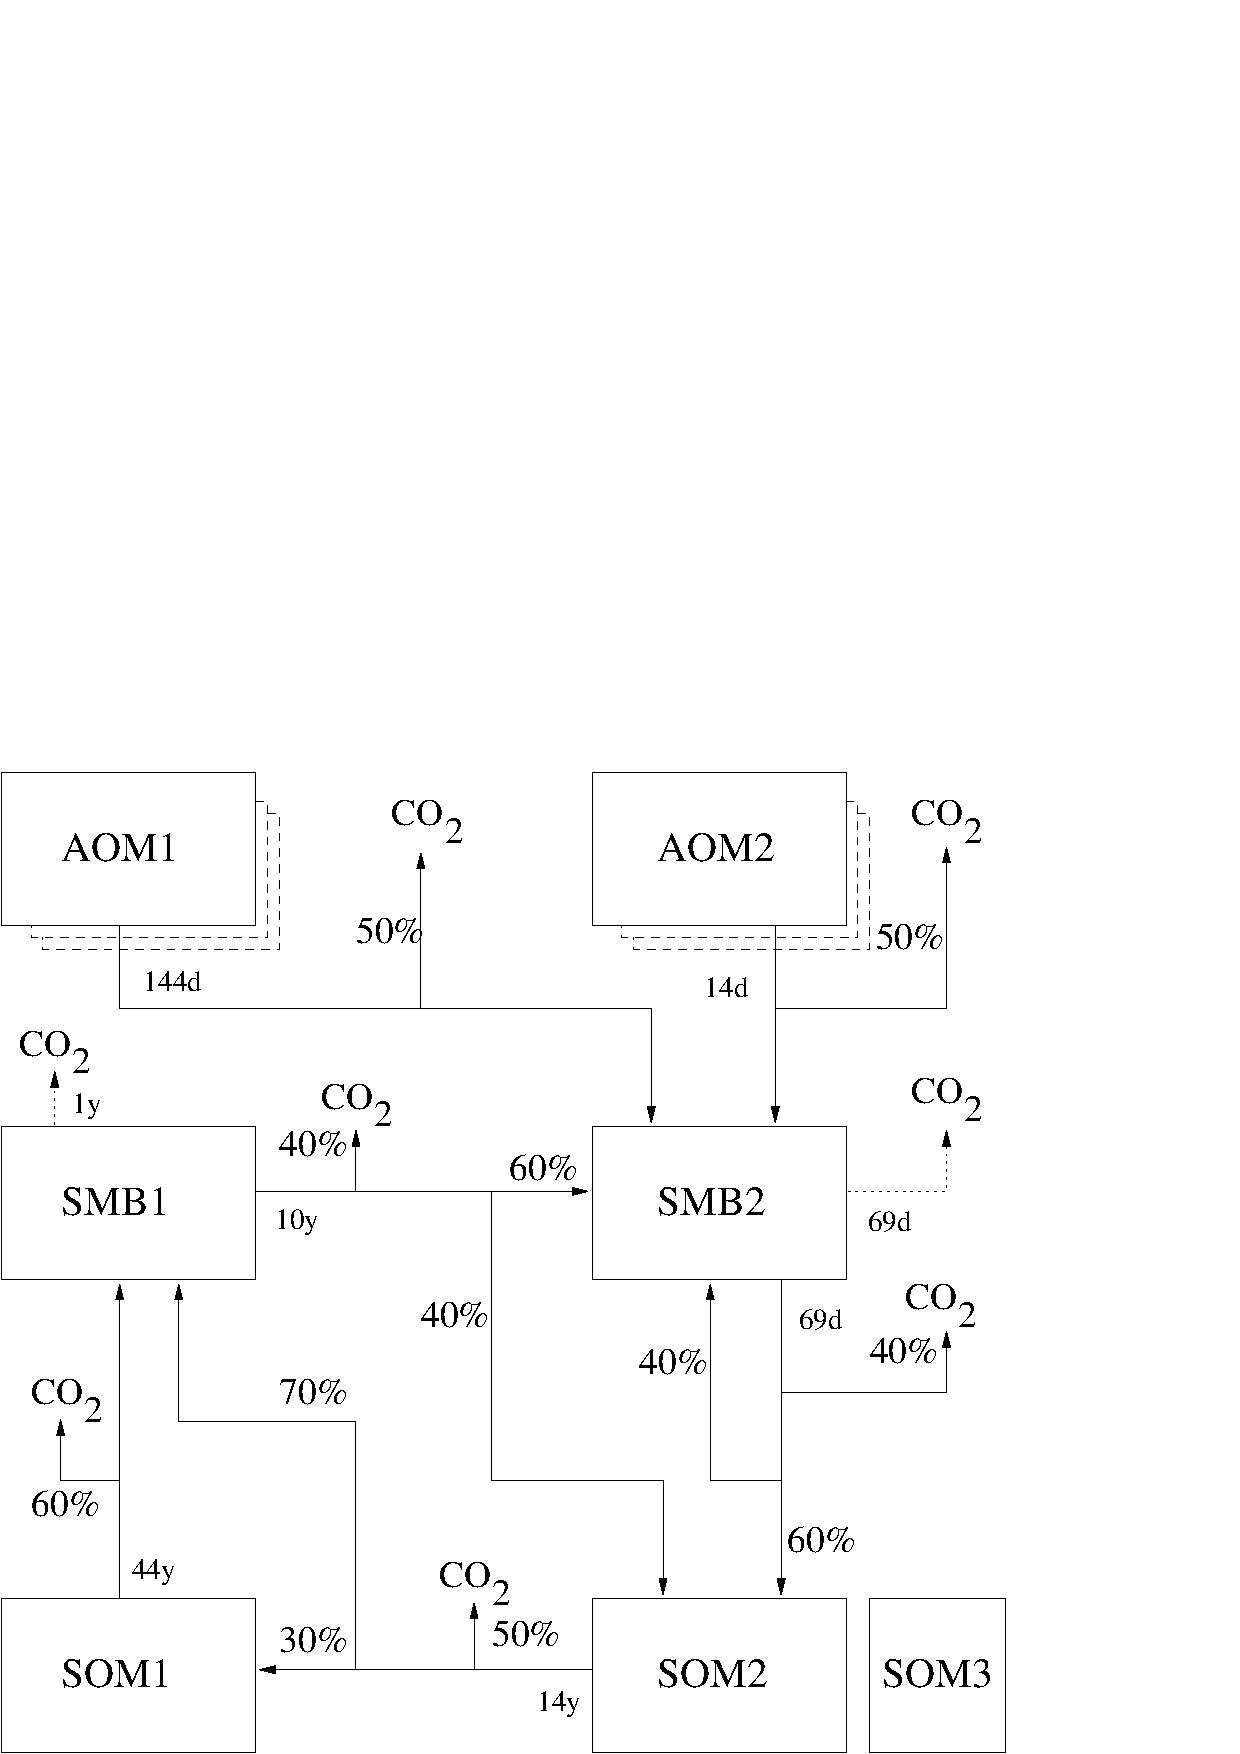
\includegraphics[width=\columnwidth]{om2}
    %%\input{om2}
  \end{center}
  \caption{Current standard organic matter model in Daisy.}
  \label{fig:om2}
\end{figure}

The amount of carbon turned over and decomposed is directly
proportional with the size of the pool. We call this the
\emph{turnover rate} by the soil microbial biomass. All the pools in
Fig.~\ref{fig:om2} have a fully drawn outgoing line. From the
\textsc{som1} pool the outgoing line is marked with the text
``44y''. This indicate the turnover rate of this particular pool and
the number is the corresponding halftime (defined as $\ln 2/k$, where
$k$ is the turnover rate.  For this model, the halftime is 44 years
for the \textsc{som1} pool), which means that if there was no input to
the pool, the pool would be half the original size after 44 years. For
some pools this time is given in days, e.g.\ the \textsc{smb2} pool
has a turnover halftime of 69 days.

If we follow the line from \textsc{som1} it splits into two
parts. 60\% is completely mineralized and lost as CO$_2$, the rest is
allocated to the microbial biomass in the \textsc{smb1}
pool. Considering the \textsc{som2} pool, we see that 70\% of the
carbon not lost as CO$_2$, are allocated to the microbial biomass and
the remaining 30\% ends up in \textsc{som1}. Besides a turnover rate,
the two \textsc{smb} pools also have a maintenance rate. This rate
reflects the cost of staying alive, and is indicated by a stippled
line out of the \textsc{smb} pools. In general, both the rates and the
number of \textsc{aom} pools are variable; the rates given here are
just examples. Also, there can be many sets of added organic matter
pools, each set corresponds to a particular fertilizer or residual
with its specific parameters.

The turnover and maintenance of the pools is affected by abiotic
factors, namely the clay content in the soil, the soil temperature,
and the moisture. The halftimes listed in Fig.~\ref{fig:om2}
corresponds to 0\% clay, 10$^\circ$C, and field capacity (defined as
-100 hPa). The halftimes will increase with increasing clay content,
decreasing temperature, and decreasing soil water content, as seen on
Fig.~\ref{fig:abiotic}. Further information of the abiotic factors
included in the organic matter model in Daisy is given in
\citet{daisy-def}.

\begin{figure}[htbp]
  \begin{center}
  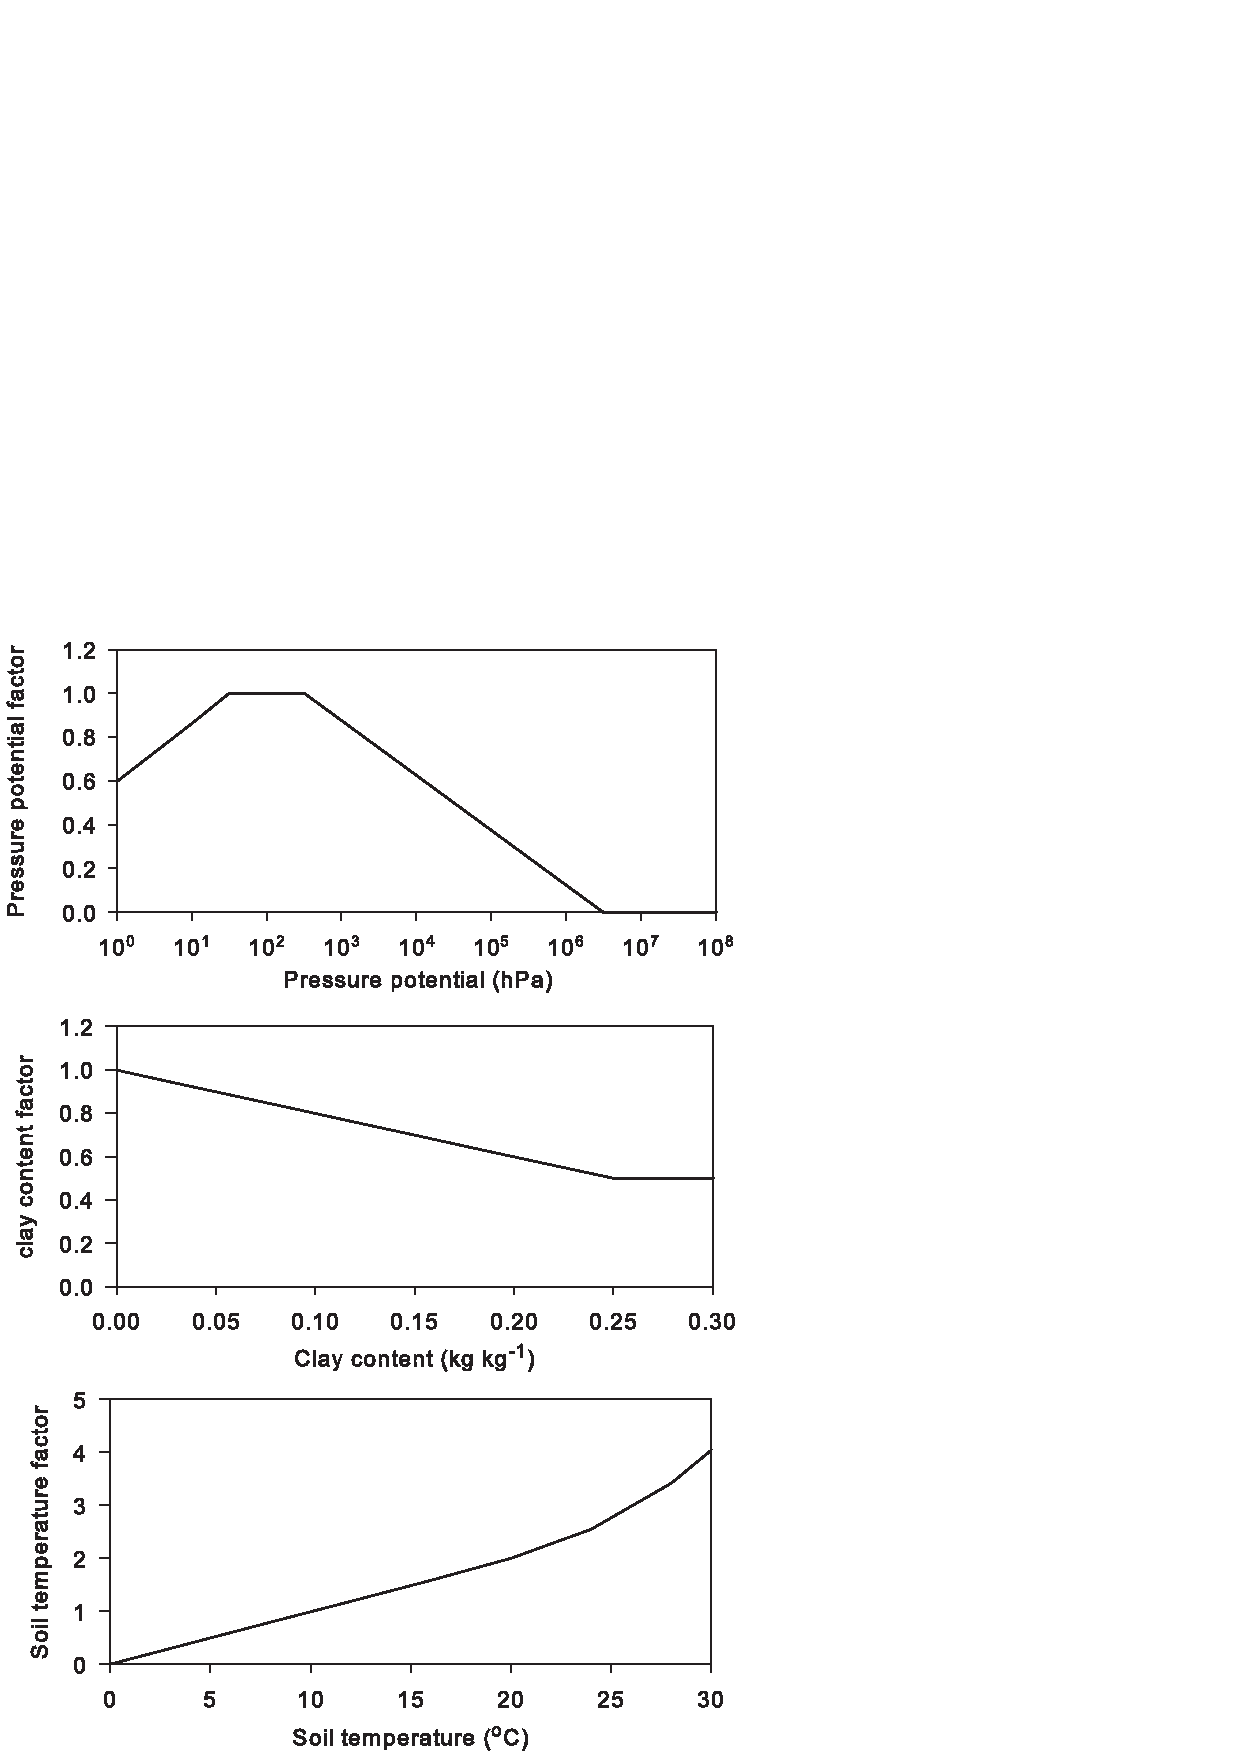
\includegraphics[width=\columnwidth]{abiotic}
  \end{center}
  \caption{Effect of abiotic factors on turnover.}
  \label{fig:abiotic}
\end{figure}

\section{Initialization of the organic matter pools}

Initialization of the partition of the organic matter into the various
soil pools have been a particular stumbling block for most users,
partly because the partition does not reflect an easily identifiable
property of the system being modeled.  This lead to the development of
a subsystem for initialization of the organic matter pools based on a
static approximation of the dynamic model, which will be explored in
the next section.

Daisy provides several methods for initialization of the organic
matter pools.  The largest amount of control can be achieved by
explicitly specifying the content of each pool.  However, since this
requires far more information of both the soil and the model than the
user can reasonably be expected to possess, this initialization option
is almost exclusively used for hotstarts, that is, restarting the
simulation from the saved state of an earlier simulation.  Instead, a
static approximation of the dynamic organic matter turnover model is
used in order to simplify the initialization.

The organic matter model is dynamic due to the uneven application of
\textsc{aom}, and the weather dependent abiotic factors.  The static
model is achieved by considering average input of added organic
matter, and effective static values for the abiotic factors.  If we
assume the dynamic model is not strongly dependent of the initial
conditions, we can combine this initial estimate with a warmup period,
to achive a reasonable initial state for the period we are interested
in simulating.

For typical use of Daisy (agricultural soil with annual crops) this
works well for the initialization of the \textsc{smb} and \textsc{aom}
pools.  After one or two years, the \textsc{smb} and \textsc{aom}
pools will have adjusted to level of input, and the earlier history
will be less relevant.  However, as shall be demonstrated in
Sect.~\ref{sec:results}, the \textsc{som} pools can take centuries
to reach equilibrium with new input levels.

\subsection{Generalized equations}

The rate of change of the individual pools in the dynamic model is
governed by Eq.~(\ref{eq:generic}).
\begin{equation}
  \label{eq:generic}
  \begin{array}{lcll}
    \Delta\mbox{\textsc{smb}}i &=& \displaystyle
    \sum_{j=1}^{\nsom} a_{i,j}\,\mbox{\textsc{smb}}j +
    \sum_{j=1}^{\nsom} b_{i,j}\,&\mbox{\textsc{som}}j\\
    & & + \sum_{j=1}^{\naom} c_{i,j}\,\mbox{\textsc{aom}}j
    &;i = 1\ldots \nsmb\\
    \Delta\mbox{\textsc{som}}i &=& \displaystyle
    \sum_{j=1}^{\nsmb} d_{i,j}\,\mbox{\textsc{smb}}j +
    \sum_{j=1}^{\nsom} e_{i,j}\,&\mbox{\textsc{som}}j\\
    & & + \sum_{j=1}^{\naom} f_{i,j}\,\mbox{\textsc{aom}}j
    &;i = 1\ldots \nsom\\
    \Delta\mbox{\textsc{aom}}i &=& \displaystyle g_i\,\mbox{\textsc{aom}}i
    &;i = 1\ldots \naom\\
  \end{array}
\end{equation}
Here, \textsc{aom}$i$, \textsc{smb}$i$, and \textsc{som}$i$ denote the
carbon content (mass) of the $i$'th \textsc{smb}, \textsc{som}, or
\textsc{aom} pool, respectively.  $\Delta\mbox{\textsc{aom}}i$,
$\Delta\mbox{\textsc{smb}}i$, and $\Delta\mbox{\textsc{som}}i$ denote
the change of each pool (mass per time).  $\naom$,
$\nsmb$, and $\nsom$ denote the number of
\textsc{aom}, \textsc{smb} and \textsc{som} pools, respectively.

The relationship between the mass of the pools, and the change of the
pools, is assumed to be linear, and denoted by $a_{i,j}$, $b_{i,j}$,
$c_{i,j}$, $d_{i,j}$, $e_{i,j}$, $f_{i,j}$ and $g_i$ (fraction per time)
respectively.  These relationships are calculated on basis of the
parametrization of the organic matter turnover model.  For example,
the formula for finding $a_{1,2}$ can be found in
Eq.~(\ref{eq:a12}).
\begin{equation}
  \label{eq:a12}
  \begin{array}{rcl}
  a_{1,2} & = & (t_{\mbox{\tiny\textsc{smb1}}}\,
  (X_{\mbox{\tiny\textsc{smb1}}\rightarrow{\mbox{\tiny\textsc{smb2}}}}\,
  E_{\mbox{\tiny\textsc{smb1}}}
  - 1) - m_{\mbox{\tiny\textsc{smb1}}})\\
  & & F_{\mbox{\tiny\textsc{smb1}}}^T (T)\,
  F_{\mbox{\tiny\textsc{smb1}}}^\psi (\psi)\,
  F_{\mbox{\tiny\textsc{smb1}}}^C (X_c)
  \end{array}
\end{equation}
Where $t_{\mbox{\tiny\textsc{smb1}}}$ is the turnover rate and
$m_{\mbox{\tiny\textsc{smb1}}}$ is the maintenance of the
\textsc{smb1}
pool. $X_{\mbox{\tiny\textsc{smb1}}\rightarrow{\mbox{\tiny\textsc{smb2}}}}$
is the carbon fraction going from \textsc{smb1} to
\textsc{smb2}. $E_{\mbox{\tiny\textsc{smb1}}}$ is the efficiency of
which \textsc{smb1} can be decomposed, the remaining part is lost to
the atmosphere as CO$_2$. $F_{\mbox{\tiny\textsc{smb1}}}^T$,
$F_{\mbox{\tiny\textsc{smb1}}}^\psi$, and
$F_{\mbox{\tiny\textsc{smb1}}}^C$ are functions describing the effect
of the abiotic factors for soil temperature, moisture, and clay,
respectively. The other relationships in Eq.~(\ref{eq:generic})
can be described by similar forms.

\subsection{Known and unknowns}

For initialization purposes, we assume that the temperature and soil
humidity are constant and known, which means $a_{i,j}$, $b_{i,j}$,
$c_{i,j}$, $d_{i,j}$, $e_{i,j}$, $f_{i,j}$ and $g_i$ will also all be
known constants. This still leaves us with one equation, and two
unknowns (content and change) for each pool in our system.  In order
to find a solution, we will need further assumptions to either
increase the number of equations, or decrease the number of unknowns.

\subsection{Initialization methods}

The Daisy software provides the user with six methods for
initialization, each will result in a linear equation system that can
be solved using a standard technique (Gauss-Jordan elimination is used
in Daisy). The methods will be listed in the following sections.  All
the methods rely on the assumtion that the \textsc{smb} pools are in
equilibrium, meaning $\Delta\mbox{\textsc{smb}}i$ are all zero
Eq.~(\ref{eq:smb-eq}).
\begin{equation}
  \label{eq:smb-eq}
  \Delta\mbox{\textsc{smb}}i = 0 \hspace{1cm};i = 1\ldots \nsmb
\end{equation}
This is reasonable as the \textsc{smb} pools tend to adjust to input
levels relatively fast (a few years at most).  All but one
initialization option require the user to specify the total organic
matter in the soil, which allows us to add Eq.~(\ref{eq:total}) to
the system without increasing the number of unknowns.
\begin{equation}
  \label{eq:total}
  \mbox{\textsc{tom}} = \sum_{i=1}^{\nsmb} \mbox{\textsc{smb}}i
    + \sum_{i=1}^{\nsom} \mbox{\textsc{som}}i
    + \sum_{i=1}^{\naom} \mbox{\textsc{aom}}i
\end{equation}
The final common assumption is that the carbon input is known, as in
Eq.~(\ref{eq:input}).
\begin{equation}
  \label{eq:input}
  \Delta\mbox{\textsc{aom}}i = k_i \hspace{1cm};i = 1\ldots \naom
\end{equation}
Here $k_i$ denote the known carbon input to \textsc{aom}$i$, from
which the size of \textsc{aom}$i$ can trivially be found given
Eq.~(\ref{eq:generic}) ($\mbox{\textsc{aom}}i = k_i / g_i$), and
eliminated as unknowns from the equation system.

Combining all three assumptions, we still lack
$\nsom-1$ equations before we can solve the system.

\subsection{Method 1: Explicit SOM partitioning}

The original, and still supported, method of initializing the
\textsc{som} pools was to require the user to explicitly specify the
fraction of the total \textsc{som} allocated to each pool, at in
Eq.~(\ref{eq:som-fractions}).
\begin{equation}
  \label{eq:som-fractions}
  \mbox{\textsc{som}}i = f_{\mbox{\scriptsize\textsc{som}}i} 
    \sum_{j=1}^{\nsom} \mbox{\textsc{som}}j
    \hspace{1cm};i = 1\ldots \nsom
\end{equation}
where $f_{\mbox{\scriptsize\textsc{som}}i}$ are user supplied
fractions.  This gives us $\nsom$ additional equations, however since
$\sum_{i=1}^{\nsom} f_{\mbox{\scriptsize\textsc{som}}i} = 1$ the
system is overspecified, and we leave out one of the equations.  That
is, for a system with two \textsc{som} pools, we only specify one
equation, $\mbox{\textsc{som}}1 = f_{\mbox{\scriptsize\textsc{som}}1}
(\mbox{\textsc{som}}1 + \mbox{\textsc{som}}2)$.  Thus,
Eqs.~(\ref{eq:som-fractions}), (\ref{eq:smb-eq}), (\ref{eq:total}),
and (\ref{eq:input}) this gives us enough equations to find a
solution.

The explicit \textsc{som} partitioning gives the user good control
over the simulation with a manageable number of parameters.  However,
the \textsc{som} partitioning is model specific, and does not
correspond to measurable quantities.  

\subsection{Method 2: Background mineralization}

For simulations where our main interest is in the soil organic matter
as a nitrogen storage, Daisy allow the user to specify desired
background mineralization levels.  The background mineralization is
defined as the decrease over time of nitrogen stored in the
\textsc{som} pools.  Assuming a constant C/N ratio for each pool
($\mbox{\textsc{c/n}}_{\mbox{\scriptsize\textsc{som}}i}$), gives us the equation
\begin{equation}
  \label{eq:cn}
  background = \sum_{i=1}^{\nsom}
  \frac{\Delta\mbox{\textsc{som}}i}
       {\mbox{\textsc{c/n}}_{\mbox{\scriptsize\textsc{som}}i}}
\end{equation}
This gives us one extra equation.  In the case of two \textsc{som}
pools, we then have enough equations to find a solution.  Using
background mineralization for initializing the system has the
advantages of being model independent and even indirectly measurable,
but requires a good understanding of the nitrogen dynamics of the
system.

\subsection{Equilibrium assumptions}

If the system is in equilibrium, none of the pools will change, so we
can add Eq.~(\ref{eq:som-eq}).
\begin{equation}
  \label{eq:som-eq}
  \Delta\mbox{\textsc{som}}i = 0 \hspace{1cm};i = 1\ldots \nsom
\end{equation}
Together with Eqs.~(\ref{eq:smb-eq}), (\ref{eq:total}), and
(\ref{eq:input}) this gives us one more equation than needed, so Daisy
will allow the user to relax some other assumption.  This leads to the
three different variants explained in the following.

\subsubsection{Method 3: Size of inert pool}

If we have an inert pool, like \textsc{som3} in Fig.~\ref{fig:om2},
adding an equation stating that $\Delta\mbox{\textsc{som}}3 = 0$
does not add any additional information (it is already part of
Eq.~(\ref{eq:generic}), where $d_{3,j}$, $e_{3,j}$, and $f_{3,j}$ will
be $0$ for all $j$).  This is the case for the default initialization
of the subsoil, here we assume the active pools are in equilibrium
with the input, and let the equation system find the size of the inert
pool.

\subsubsection{Method 4: Total organic matter}

The second equilibrium initialization allows the user to leave out
Eq.~(\ref{eq:total}), so the total amount of (active) soil organic
matter is estimated from the input levels.  This is rarely useful, as
total amount of organic material is easy to measure, but has been used
in this paper to initialize the organic matter content for long term
simulations in section~\ref{sec:simulations}, where we examine the
period from one equilibrium to another.

\subsubsection{Method 5: Unknown input}

The last and most common equilibrium initialization is to let the user
specify the size of the inert pool (usually to zero), and leave out
Eq.~(\ref{eq:input}).  This is useful for cases where the user have
no idea of what the input levels for the field used to be.

\subsection{Method 6: Quasi-equilibrium}

The default initialization for organic matter in the plough layer is
to weaken the equilibrium assumption, and allow the pool with the
lowest (non-zero) turnover rate to change.  That is, we remove one of
the equations added by Eq.~(\ref{eq:som-eq}), namely for the slowest
active pool, typically \textsc{som1}, and keep all of
Eqs.~(\ref{eq:smb-eq}), (\ref{eq:total}), and (\ref{eq:input}).  The idea is
that all the fast pools will quickly adapt to the input and to the
size of the slow pool.

\section{Simulations}
\label{sec:simulations}

In this section, we compare the static solutions we get with the
equilibrium and the quasi-equilibrium assumptions from the previous
section, using a dynamic simulation as a baseline, and the model
described in Sect.~\ref{sec:model} with an empty \textsc{som3} pool. In
the dynamic simulations we follow a system that goes from equilibrium
at one level of carbon input, to equilibrium at another input level.
In particular we follow the relative size of the two active
\textsc{som} pools.

\subsection{Driving variables and soil parameters}

Since the organic matter paramterization in Daisy has been developed
based on Danish soils, we have used Danish data for all simulations.

\subsubsection{Weather}

The weather data are from an meteorological research station in
Taastrup, in the Eastern part of Denmark.  A time series from 1970 to
1999 was used, and was repeated for the entire simulation.  The
simulation period was 600 years.

\subsubsection{Soil}

To include the effect of clay content, two standard soils for Danish
conditions have been selected, a coarse sand typical for the Western
part of Denmark, and a sandy loam typical for the Eastern parts of
Denmark.  The particle size distribution and dry bulk density $\rho_b$
of the two soils are listed in Table~\ref{tab:psd}.
\begin{table}[htbp]
  \caption{Particle size distribution and dry bulk density $\rho_b$ of
    the two standard soils.} 
  \label{tab:psd}
  \vspace{0.25cm}
  \begin{tabular}{c c c c c}
    \hline
    Soil        &  clay     & silt        & sand           & $\rho_b$ \\
                & (<2 $�$m) & (2-50 $�$m) & (50-2000 $�$m) & g/cm$^3$ \\\hline
    Sand        & 3.9       & 6.4         & 89.7           & 1.45 \\
    Sandy loam  & 12.4      & 24.9        & 62.7           & 1.53 \\\hline
  \end{tabular}
\end{table}
The total organic matter is not listed, as we initialize it to be in
equilibrium with the specified input.  Only the plow layer (0--30
cm) is considred in the simulations.

\subsubsection{Management}

Two management practice of high and low C-input to the simulated
systems have been evaluated for each soil. For the coarse sand also a
medium C-input management was included. All the management practices
have been taken from \citet{daisy-staabi}. Table~\ref{tab:soils} lists
the average C-input together with the average and initial abiotic
factor and the initial C-input of the different management and soil
combinations.
\begin{table}[htbp]
  \caption{Average input of organic C to thw plow layer (0--30 cm) and
    average abiotic factor (heat factor times humidity factor) in
    simulated management for sandy and sandy loam soils. The initial
    abiotic factor and initial C refers to the initialization of the
    organic matter module using equilibrium assumptions.  The unit for
    C input is kg C ha$^{-1}$ y$^{-1}$.  The average abiotic factor
    was also used for initialization, thus only one number is listed
    in the table.}
  \label{tab:soils}
\vspace{0.25cm}
\begin{tabular}{c c c c c c}
  \hline
        &            & average & abiotic & initial & initial\\
  Soil  & Manag.     & C input & factor  & C input & \textsc{tom} \\\hline
  Sand  & Low        & 1817    & 0.680   & 5200 & ? \\
  Sand  & Medium     & 4412    & 0.680   & 5200 & ? \\
  Sand  & High       & 5158    & 0.681   & 1800 & ? \\
  Sandy loam & Low   & 2283    & 0.622   & 6500 & ? \\
  Sandy loam & High  & 6525    & 0.623   & 2300 & ?\\\hline
\end{tabular}
\end{table}
The total C input is higher in the sandy loam soil than in the sandy
soil because crop production is higher, which results in a higher
input of residuals.

\subsubsection{Abiotic factors}

For the initialization we must use constant values.  This is not a
problem for clay, which varies little within the time frames we are
concerned with, but problematic for the temperature and hummidity
effects.  By default the Daisy model use the local average air
temperature (which is already specified by the user in the weather
file) for $T$, and field capacity (-100 hPa) for the water potential. A
better estimate can be achieved by logging the product of factors in a
realistic simulation.

Figure~\ref{fig:year} shows the variation of the product of the heat
and humidity effects within a specific year for both the sand, and the
sandy loam.  The abiotic factors for the two soils are equal during
the winther, where the humidity is high enough that only the
temperature has an effect.  This is typical for Danish conditions.
During the summer, the sand gets dryer than the sandy loam, so the
combined factor is also lower.
\begin{figure}[htbp]
  \begin{tabular}{l}
    Abiotic factor\\
    \hspace{-1.5cm}% GNUPLOT: LaTeX picture with Postscript
\begingroup
  \makeatletter
  \providecommand\color[2][]{%
    \GenericError{(gnuplot) \space\space\space\@spaces}{%
      Package color not loaded in conjunction with
      terminal option `colourtext'%
    }{See the gnuplot documentation for explanation.%
    }{Either use 'blacktext' in gnuplot or load the package
      color.sty in LaTeX.}%
    \renewcommand\color[2][]{}%
  }%
  \providecommand\includegraphics[2][]{%
    \GenericError{(gnuplot) \space\space\space\@spaces}{%
      Package graphicx or graphics not loaded%
    }{See the gnuplot documentation for explanation.%
    }{The gnuplot epslatex terminal needs graphicx.sty or graphics.sty.}%
    \renewcommand\includegraphics[2][]{}%
  }%
  \providecommand\rotatebox[2]{#2}%
  \@ifundefined{ifGPcolor}{%
    \newif\ifGPcolor
    \GPcolortrue
  }{}%
  \@ifundefined{ifGPblacktext}{%
    \newif\ifGPblacktext
    \GPblacktexttrue
  }{}%
  % define a \g@addto@macro without @ in the name:
  \let\gplgaddtomacro\g@addto@macro
  % define empty templates for all commands taking text:
  \gdef\gplbacktext{}%
  \gdef\gplfronttext{}%
  \makeatother
  \ifGPblacktext
    % no textcolor at all
    \def\colorrgb#1{}%
    \def\colorgray#1{}%
  \else
    % gray or color?
    \ifGPcolor
      \def\colorrgb#1{\color[rgb]{#1}}%
      \def\colorgray#1{\color[gray]{#1}}%
      \expandafter\def\csname LTw\endcsname{\color{white}}%
      \expandafter\def\csname LTb\endcsname{\color{black}}%
      \expandafter\def\csname LTa\endcsname{\color{black}}%
      \expandafter\def\csname LT0\endcsname{\color[rgb]{1,0,0}}%
      \expandafter\def\csname LT1\endcsname{\color[rgb]{0,1,0}}%
      \expandafter\def\csname LT2\endcsname{\color[rgb]{0,0,1}}%
      \expandafter\def\csname LT3\endcsname{\color[rgb]{1,0,1}}%
      \expandafter\def\csname LT4\endcsname{\color[rgb]{0,1,1}}%
      \expandafter\def\csname LT5\endcsname{\color[rgb]{1,1,0}}%
      \expandafter\def\csname LT6\endcsname{\color[rgb]{0,0,0}}%
      \expandafter\def\csname LT7\endcsname{\color[rgb]{1,0.3,0}}%
      \expandafter\def\csname LT8\endcsname{\color[rgb]{0.5,0.5,0.5}}%
    \else
      % gray
      \def\colorrgb#1{\color{black}}%
      \def\colorgray#1{\color[gray]{#1}}%
      \expandafter\def\csname LTw\endcsname{\color{white}}%
      \expandafter\def\csname LTb\endcsname{\color{black}}%
      \expandafter\def\csname LTa\endcsname{\color{black}}%
      \expandafter\def\csname LT0\endcsname{\color{black}}%
      \expandafter\def\csname LT1\endcsname{\color{black}}%
      \expandafter\def\csname LT2\endcsname{\color{black}}%
      \expandafter\def\csname LT3\endcsname{\color{black}}%
      \expandafter\def\csname LT4\endcsname{\color{black}}%
      \expandafter\def\csname LT5\endcsname{\color{black}}%
      \expandafter\def\csname LT6\endcsname{\color{black}}%
      \expandafter\def\csname LT7\endcsname{\color{black}}%
      \expandafter\def\csname LT8\endcsname{\color{black}}%
    \fi
  \fi
  \setlength{\unitlength}{0.0500bp}%
  \begin{picture}(5760.00,3024.00)%
    \gplgaddtomacro\gplbacktext{%
      \csname LTb\endcsname%
      \put(1034,1144){\makebox(0,0)[r]{\strut{} 0}}%
      \put(1034,1359){\makebox(0,0)[r]{\strut{} 0.2}}%
      \put(1034,1575){\makebox(0,0)[r]{\strut{} 0.4}}%
      \put(1034,1790){\makebox(0,0)[r]{\strut{} 0.6}}%
      \put(1034,2006){\makebox(0,0)[r]{\strut{} 0.8}}%
      \put(1034,2221){\makebox(0,0)[r]{\strut{} 1}}%
      \put(1034,2437){\makebox(0,0)[r]{\strut{} 1.2}}%
      \put(1034,2652){\makebox(0,0)[r]{\strut{} 1.4}}%
      \put(1166,924){\makebox(0,0){\strut{}01}}%
      \put(1542,924){\makebox(0,0){\strut{}02}}%
      \put(1894,924){\makebox(0,0){\strut{}03}}%
      \put(2257,924){\makebox(0,0){\strut{}04}}%
      \put(2622,924){\makebox(0,0){\strut{}05}}%
      \put(2985,924){\makebox(0,0){\strut{}06}}%
      \put(3349,924){\makebox(0,0){\strut{}07}}%
      \put(3713,924){\makebox(0,0){\strut{}08}}%
      \put(4089,924){\makebox(0,0){\strut{}09}}%
      \put(4453,924){\makebox(0,0){\strut{}10}}%
      \put(4817,924){\makebox(0,0){\strut{}11}}%
      \put(5181,924){\makebox(0,0){\strut{}12}}%
      \put(484,1952){\rotatebox{90}{\makebox(0,0){\strut{}}}}%
      \put(3342,594){\makebox(0,0){\strut{}Month}}%
    }%
    \gplgaddtomacro\gplfronttext{%
      \csname LTb\endcsname%
      \put(2487,173){\makebox(0,0)[r]{\strut{}JB1}}%
      \csname LTb\endcsname%
      \put(3738,173){\makebox(0,0)[r]{\strut{}JB6}}%
    }%
    \gplbacktext
    \put(0,0){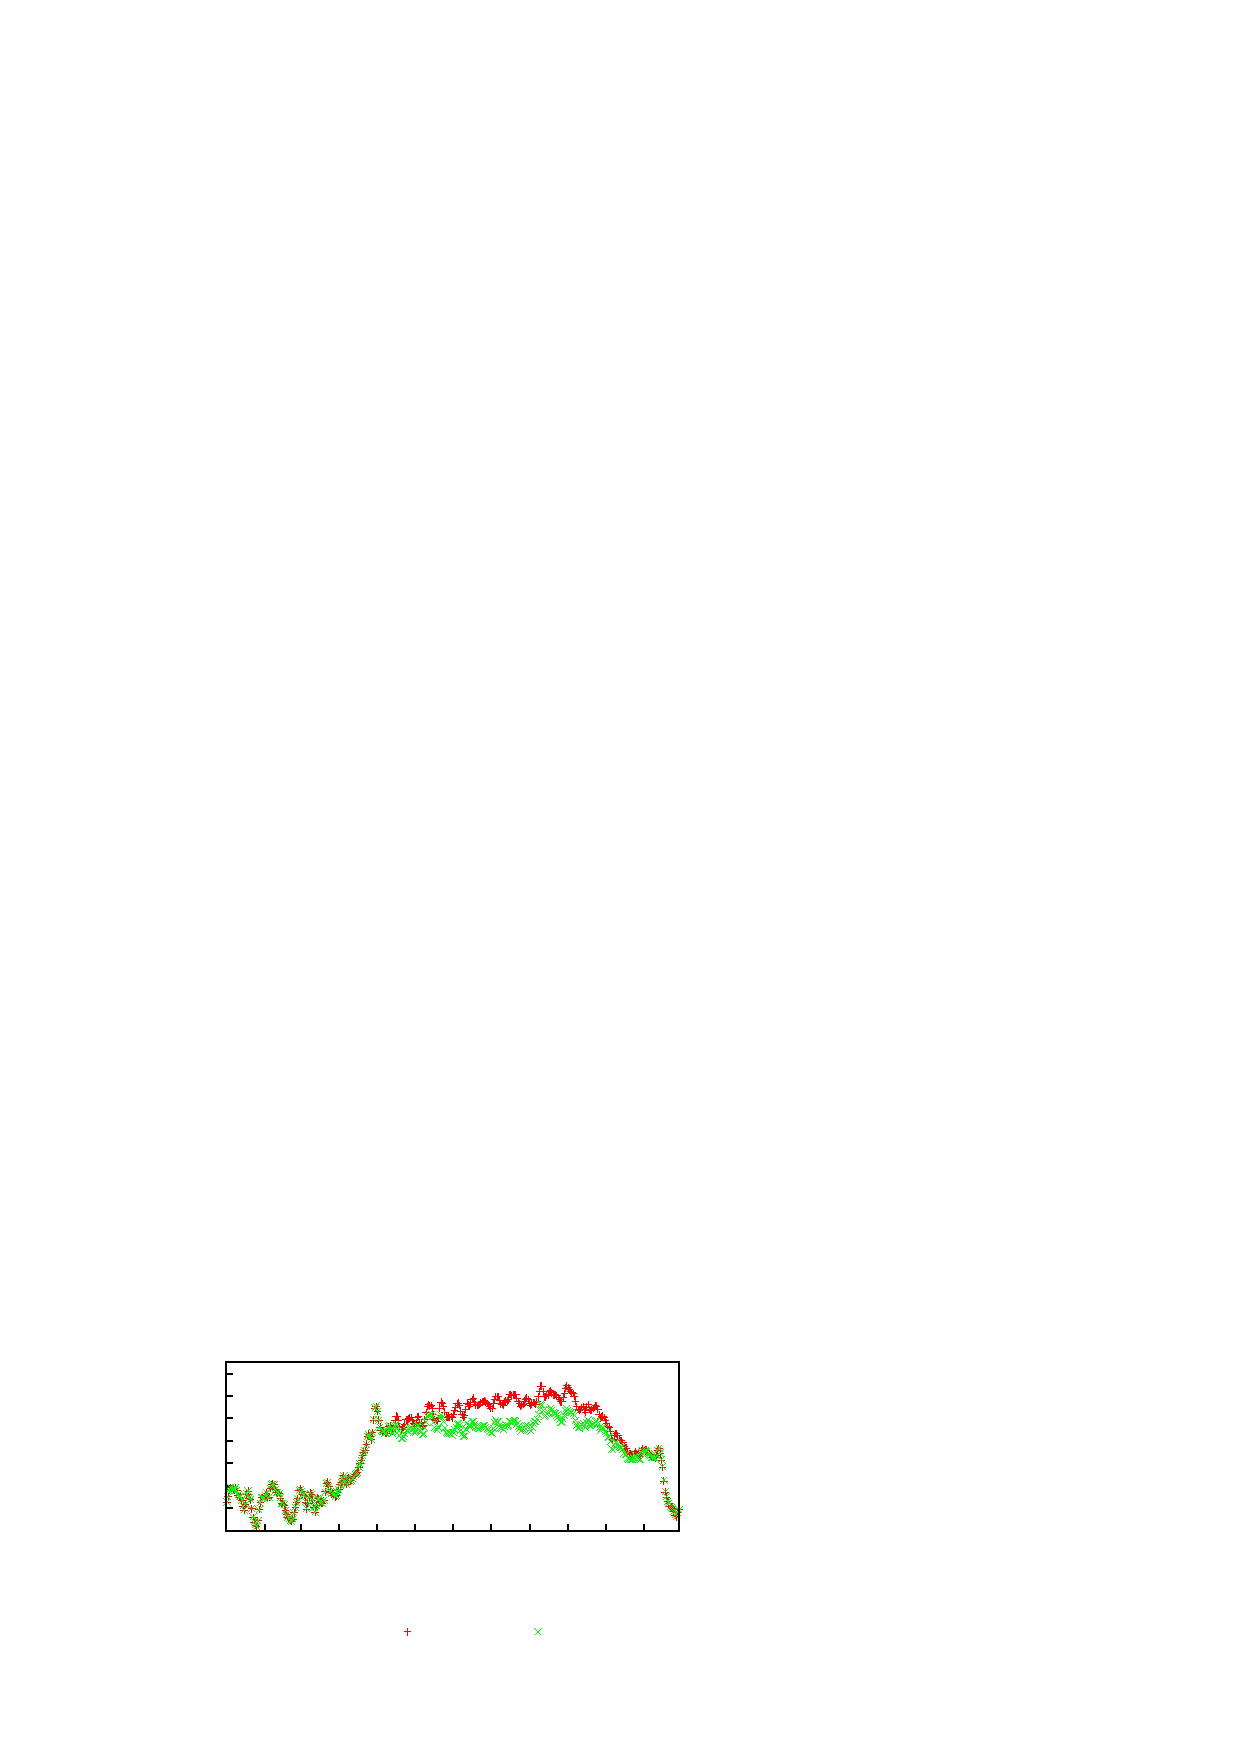
\includegraphics{abioticYear}}%
    \gplfronttext
  \end{picture}%
\endgroup

  \end{tabular}
  \caption{The combined heat and humidity effect (y-axes) for a sand
    ($+$) and sandy loam ($\times$) as it varies over a year (x-axes).}
  \label{fig:year}
\end{figure}

Figure~\ref{fig:30} shows the variation between years of the
combined heat and hummidity effect over the 30 years of climate used,
as well as a running average.  As can be seen, at least for Danish
conditions, long time series are required before it makes sense to
talk about effective values, due to the high variation.
\begin{figure}[htbp]
  \begin{tabular}{l}
    Abiotic factor\\
    \hspace{-1.5cm}%GNUPLOT: LaTeX picture with Postscript
\begin{picture}(0,0)%

\includegraphics{abiotic30}%
\end{picture}%
\begingroup
\setlength{\unitlength}{0.0200bp}%
\begin{picture}(18000,10800)(0,0)%
\put(2200,3300){\makebox(0,0)[r]{\strut{} 0.3}}%
\put(2200,4458){\makebox(0,0)[r]{\strut{} 0.4}}%
\put(2200,5617){\makebox(0,0)[r]{\strut{} 0.5}}%
\put(2200,6775){\makebox(0,0)[r]{\strut{} 0.6}}%
\put(2200,7933){\makebox(0,0)[r]{\strut{} 0.7}}%
\put(2200,9092){\makebox(0,0)[r]{\strut{} 0.8}}%
\put(2200,10250){\makebox(0,0)[r]{\strut{} 0.9}}%
\put(2475,2750){\makebox(0,0){\strut{}2000}}%
\put(4926,2750){\makebox(0,0){\strut{}2005}}%
\put(7376,2750){\makebox(0,0){\strut{}2010}}%
\put(9826,2750){\makebox(0,0){\strut{}2015}}%
\put(12276,2750){\makebox(0,0){\strut{}2020}}%
\put(14726,2750){\makebox(0,0){\strut{}2025}}%
\put(17175,2750){\makebox(0,0){\strut{}2030}}%
\put(550,6775){\rotatebox{90}{\makebox(0,0){\strut{}Abiotic factor}}}%
\put(9825,1925){\makebox(0,0){\strut{}Year}}%
\put(5200,825){\makebox(0,0)[l]{\strut{}JB1}}%
\put(5200,275){\makebox(0,0)[l]{\strut{}JB6}}%
\put(13650,825){\makebox(0,0)[l]{\strut{}JB1-average}}%
\put(13650,275){\makebox(0,0)[l]{\strut{}JB6-average}}%
\end{picture}%
\endgroup
\endinput

  \end{tabular}
  \caption{The combined heat and humidity effect (y-axes) for a sand
    ($+$) and sandy loam ($\times$) as it varies between years
    (x-axes).  The stippled lines are the running averages for the two
    soils.}
  \label{fig:30}
\end{figure}

\subsection{Results and discussion}
\label{sec:results}

Figure~\ref{fig:long} shows the results of switching between low and
high carbon input for the two soil types.  With the organic matter
model described in Sect.~\ref{sec:model}.  Full equilibrium always
corresponds to 49\% \textsc{som1} \citep{daisy-init}, which is where
the \textsc{som1} begins and ends in all four graphs.
\begin{figure*}[htbp]
  \begin{tabular}{ll}
    \% of soil\hfill{}Sand, low input\hfill{}\% of SOM\hspace{1cm} 
    & \hspace{-0.5cm}\% of soil\hfill{}Sandy loam, low input\hfill{}\% of SOM\hspace{1.0cm} \\
    \hspace{-1.5cm}% GNUPLOT: LaTeX picture with Postscript
\begingroup
  \makeatletter
  \providecommand\color[2][]{%
    \GenericError{(gnuplot) \space\space\space\@spaces}{%
      Package color not loaded in conjunction with
      terminal option `colourtext'%
    }{See the gnuplot documentation for explanation.%
    }{Either use 'blacktext' in gnuplot or load the package
      color.sty in LaTeX.}%
    \renewcommand\color[2][]{}%
  }%
  \providecommand\includegraphics[2][]{%
    \GenericError{(gnuplot) \space\space\space\@spaces}{%
      Package graphicx or graphics not loaded%
    }{See the gnuplot documentation for explanation.%
    }{The gnuplot epslatex terminal needs graphicx.sty or graphics.sty.}%
    \renewcommand\includegraphics[2][]{}%
  }%
  \providecommand\rotatebox[2]{#2}%
  \@ifundefined{ifGPcolor}{%
    \newif\ifGPcolor
    \GPcolortrue
  }{}%
  \@ifundefined{ifGPblacktext}{%
    \newif\ifGPblacktext
    \GPblacktexttrue
  }{}%
  % define a \g@addto@macro without @ in the name:
  \let\gplgaddtomacro\g@addto@macro
  % define empty templates for all commands taking text:
  \gdef\gplbacktext{}%
  \gdef\gplfronttext{}%
  \makeatother
  \ifGPblacktext
    % no textcolor at all
    \def\colorrgb#1{}%
    \def\colorgray#1{}%
  \else
    % gray or color?
    \ifGPcolor
      \def\colorrgb#1{\color[rgb]{#1}}%
      \def\colorgray#1{\color[gray]{#1}}%
      \expandafter\def\csname LTw\endcsname{\color{white}}%
      \expandafter\def\csname LTb\endcsname{\color{black}}%
      \expandafter\def\csname LTa\endcsname{\color{black}}%
      \expandafter\def\csname LT0\endcsname{\color[rgb]{1,0,0}}%
      \expandafter\def\csname LT1\endcsname{\color[rgb]{0,1,0}}%
      \expandafter\def\csname LT2\endcsname{\color[rgb]{0,0,1}}%
      \expandafter\def\csname LT3\endcsname{\color[rgb]{1,0,1}}%
      \expandafter\def\csname LT4\endcsname{\color[rgb]{0,1,1}}%
      \expandafter\def\csname LT5\endcsname{\color[rgb]{1,1,0}}%
      \expandafter\def\csname LT6\endcsname{\color[rgb]{0,0,0}}%
      \expandafter\def\csname LT7\endcsname{\color[rgb]{1,0.3,0}}%
      \expandafter\def\csname LT8\endcsname{\color[rgb]{0.5,0.5,0.5}}%
    \else
      % gray
      \def\colorrgb#1{\color{black}}%
      \def\colorgray#1{\color[gray]{#1}}%
      \expandafter\def\csname LTw\endcsname{\color{white}}%
      \expandafter\def\csname LTb\endcsname{\color{black}}%
      \expandafter\def\csname LTa\endcsname{\color{black}}%
      \expandafter\def\csname LT0\endcsname{\color{black}}%
      \expandafter\def\csname LT1\endcsname{\color{black}}%
      \expandafter\def\csname LT2\endcsname{\color{black}}%
      \expandafter\def\csname LT3\endcsname{\color{black}}%
      \expandafter\def\csname LT4\endcsname{\color{black}}%
      \expandafter\def\csname LT5\endcsname{\color{black}}%
      \expandafter\def\csname LT6\endcsname{\color{black}}%
      \expandafter\def\csname LT7\endcsname{\color{black}}%
      \expandafter\def\csname LT8\endcsname{\color{black}}%
    \fi
  \fi
  \setlength{\unitlength}{0.0500bp}%
  \begin{picture}(6120.00,3024.00)%
    \gplgaddtomacro\gplbacktext{%
      \csname LTb\endcsname%
      \put(1034,704){\makebox(0,0)[r]{\strut{} 0}}%
      \put(1034,1047){\makebox(0,0)[r]{\strut{} 0.2}}%
      \put(1034,1389){\makebox(0,0)[r]{\strut{} 0.4}}%
      \put(1034,1732){\makebox(0,0)[r]{\strut{} 0.6}}%
      \put(1034,2075){\makebox(0,0)[r]{\strut{} 0.8}}%
      \put(1034,2417){\makebox(0,0)[r]{\strut{} 1}}%
      \put(1034,2760){\makebox(0,0)[r]{\strut{} 1.2}}%
      \put(1166,484){\makebox(0,0){\strut{}2000}}%
      \put(1841,484){\makebox(0,0){\strut{}2100}}%
      \put(2517,484){\makebox(0,0){\strut{}2200}}%
      \put(3192,484){\makebox(0,0){\strut{}2300}}%
      \put(3867,484){\makebox(0,0){\strut{}2400}}%
      \put(4543,484){\makebox(0,0){\strut{}2500}}%
      \put(5218,484){\makebox(0,0){\strut{}2600}}%
      \put(5350,704){\makebox(0,0)[l]{\strut{} 20}}%
      \put(5350,1047){\makebox(0,0)[l]{\strut{} 30}}%
      \put(5350,1389){\makebox(0,0)[l]{\strut{} 40}}%
      \put(5350,1732){\makebox(0,0)[l]{\strut{} 50}}%
      \put(5350,2075){\makebox(0,0)[l]{\strut{} 60}}%
      \put(5350,2417){\makebox(0,0)[l]{\strut{} 70}}%
      \put(5350,2760){\makebox(0,0)[l]{\strut{} 80}}%
      \put(3192,154){\makebox(0,0){\strut{}Year}}%
    }%
    \gplgaddtomacro\gplfronttext{%
    }%
    \gplbacktext
    \put(0,0){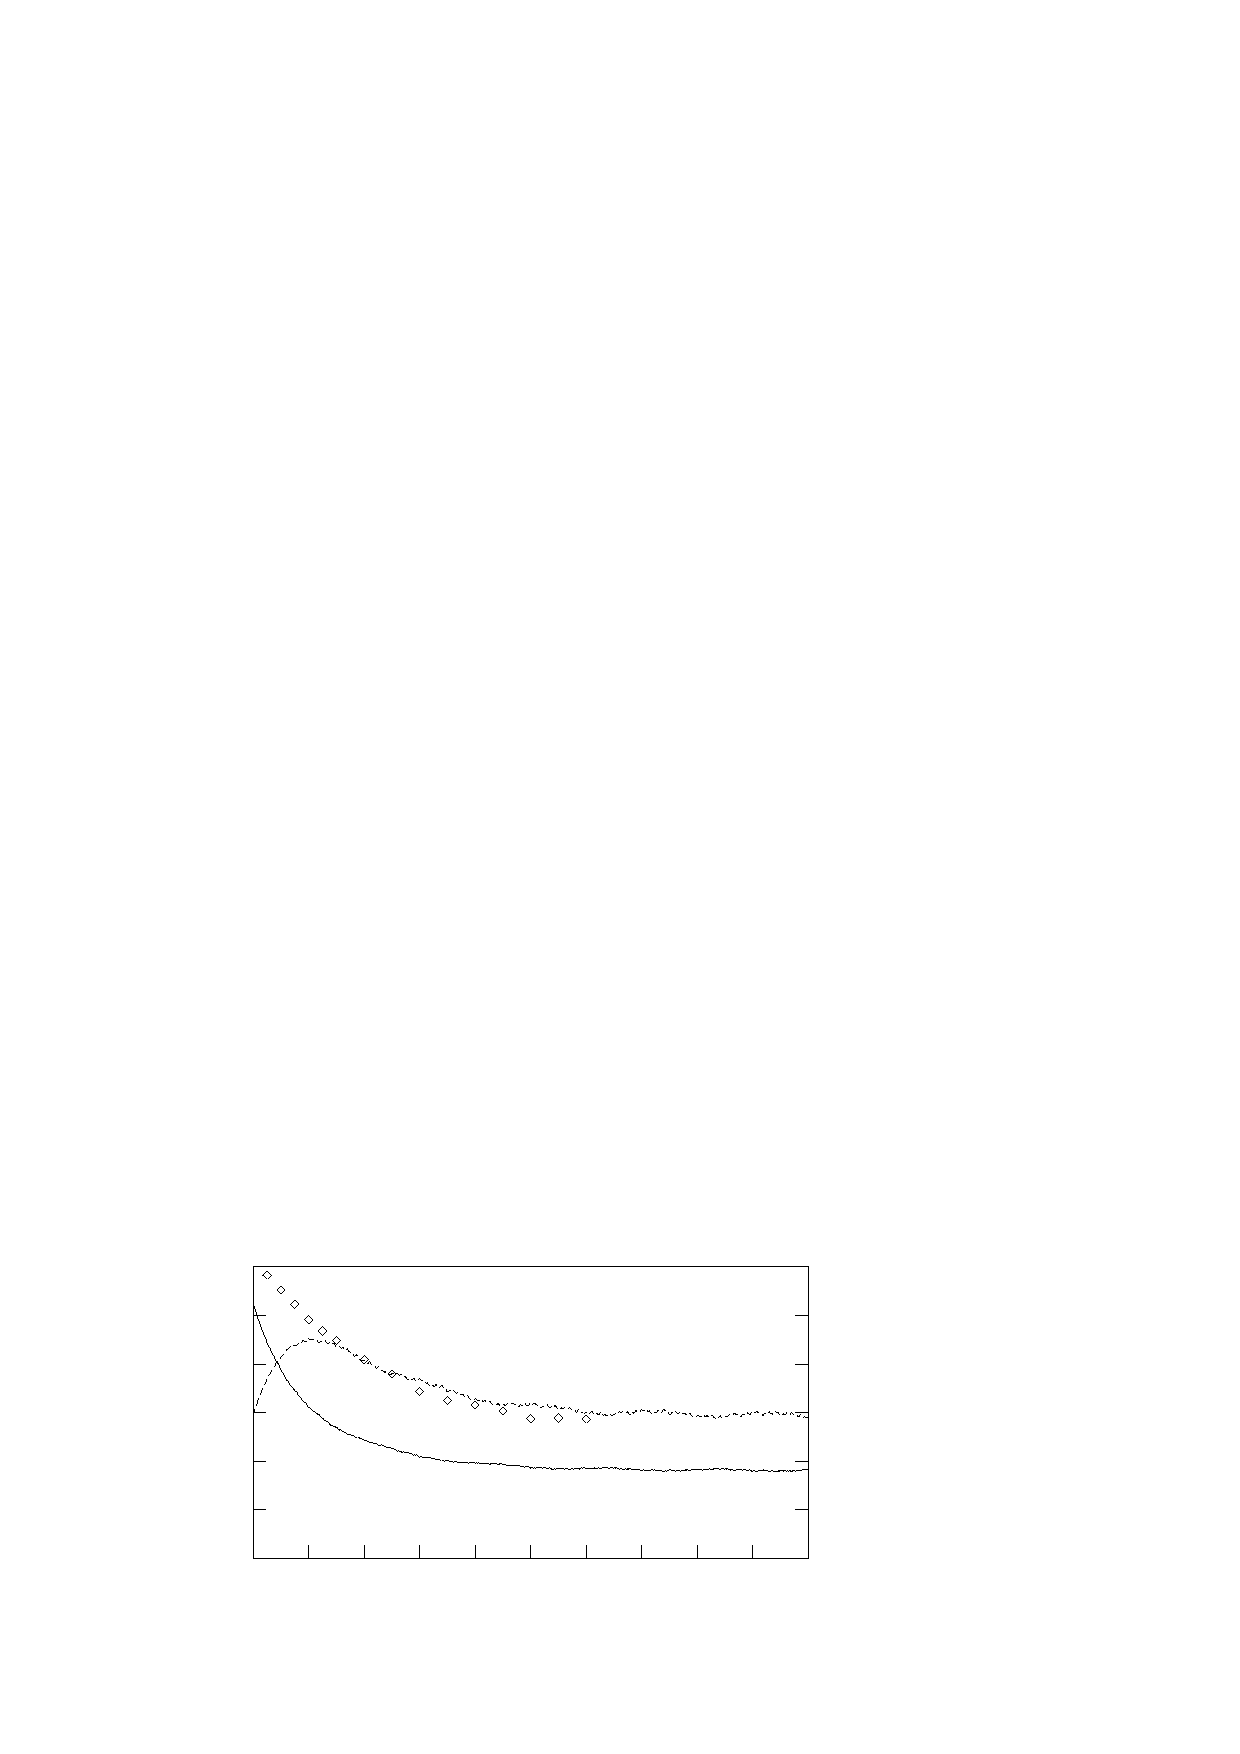
\includegraphics{realminJB6}}%
    \gplfronttext
  \end{picture}%
\endgroup
 & \hspace{-2.1cm}%GNUPLOT: LaTeX picture with Postscript
\begin{picture}(0,0)%
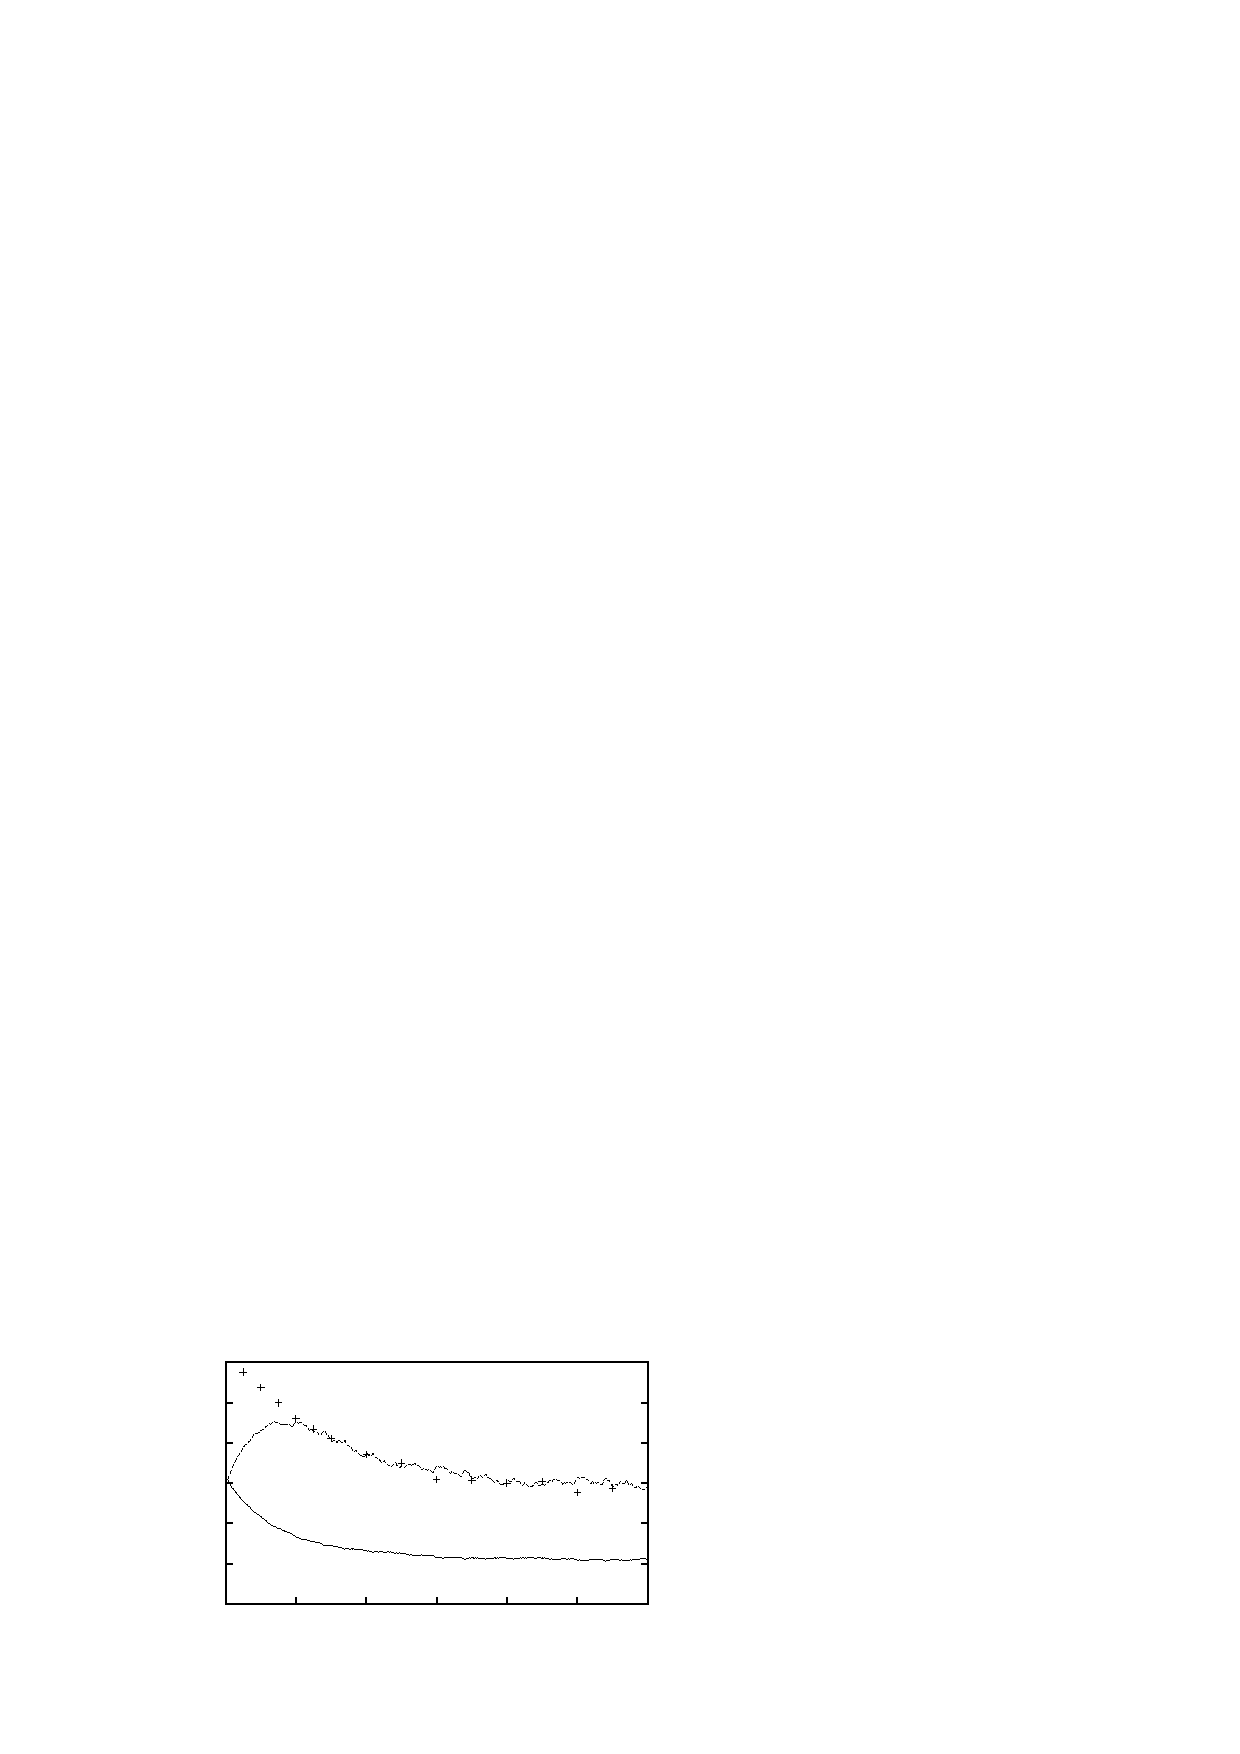
\includegraphics{realminJB1}%
\end{picture}%
\begingroup
\setlength{\unitlength}{0.0200bp}%
\begin{picture}(18000,8640)(0,0)%
\put(2200,1100){\makebox(0,0)[r]{\strut{} 0}}%
\put(2200,2265){\makebox(0,0)[r]{\strut{} 0.2}}%
\put(2200,3430){\makebox(0,0)[r]{\strut{} 0.4}}%
\put(2200,4595){\makebox(0,0)[r]{\strut{} 0.6}}%
\put(2200,5760){\makebox(0,0)[r]{\strut{} 0.8}}%
\put(2200,6925){\makebox(0,0)[r]{\strut{} 1}}%
\put(2200,8090){\makebox(0,0)[r]{\strut{} 1.2}}%
\put(2475,550){\makebox(0,0){\strut{}2000}}%
\put(3808,550){\makebox(0,0){\strut{}2100}}%
\put(5140,550){\makebox(0,0){\strut{}2200}}%
\put(6473,550){\makebox(0,0){\strut{}2300}}%
\put(7805,550){\makebox(0,0){\strut{}2400}}%
\put(9138,550){\makebox(0,0){\strut{}2500}}%
\put(10470,550){\makebox(0,0){\strut{}2600}}%
\put(11803,550){\makebox(0,0){\strut{}2700}}%
\put(13135,550){\makebox(0,0){\strut{}2800}}%
\put(14468,550){\makebox(0,0){\strut{}2900}}%
\put(15800,550){\makebox(0,0){\strut{}3000}}%
\put(16075,1100){\makebox(0,0)[l]{\strut{} 20}}%
\put(16075,2265){\makebox(0,0)[l]{\strut{} 30}}%
\put(16075,3430){\makebox(0,0)[l]{\strut{} 40}}%
\put(16075,4595){\makebox(0,0)[l]{\strut{} 50}}%
\put(16075,5760){\makebox(0,0)[l]{\strut{} 60}}%
\put(16075,6925){\makebox(0,0)[l]{\strut{} 70}}%
\put(16075,8090){\makebox(0,0)[l]{\strut{} 80}}%
\put(550,4595){\rotatebox{90}{\makebox(0,0){\strut{}Humus (\%)}}}%
\put(17449,4595){\rotatebox{90}{\makebox(0,0){\strut{}SOM1 (\%)}}}%
\end{picture}%
\endgroup
\endinput
\\
    \% of soil\hfill{}Sand, high input\hfill{}\% of SOM\hspace{1cm} 
    & \hspace{-0.5cm}\% of soil\hfill{}Sandy loam, high input\hfill{}\% of SOM\hspace{1.0cm} \\
    \hspace{-1.5cm}% GNUPLOT: LaTeX picture with Postscript
\begingroup
  \makeatletter
  \providecommand\color[2][]{%
    \GenericError{(gnuplot) \space\space\space\@spaces}{%
      Package color not loaded in conjunction with
      terminal option `colourtext'%
    }{See the gnuplot documentation for explanation.%
    }{Either use 'blacktext' in gnuplot or load the package
      color.sty in LaTeX.}%
    \renewcommand\color[2][]{}%
  }%
  \providecommand\includegraphics[2][]{%
    \GenericError{(gnuplot) \space\space\space\@spaces}{%
      Package graphicx or graphics not loaded%
    }{See the gnuplot documentation for explanation.%
    }{The gnuplot epslatex terminal needs graphicx.sty or graphics.sty.}%
    \renewcommand\includegraphics[2][]{}%
  }%
  \providecommand\rotatebox[2]{#2}%
  \@ifundefined{ifGPcolor}{%
    \newif\ifGPcolor
    \GPcolorfalse
  }{}%
  \@ifundefined{ifGPblacktext}{%
    \newif\ifGPblacktext
    \GPblacktexttrue
  }{}%
  % define a \g@addto@macro without @ in the name:
  \let\gplgaddtomacro\g@addto@macro
  % define empty templates for all commands taking text:
  \gdef\gplbacktext{}%
  \gdef\gplfronttext{}%
  \makeatother
  \ifGPblacktext
    % no textcolor at all
    \def\colorrgb#1{}%
    \def\colorgray#1{}%
  \else
    % gray or color?
    \ifGPcolor
      \def\colorrgb#1{\color[rgb]{#1}}%
      \def\colorgray#1{\color[gray]{#1}}%
      \expandafter\def\csname LTw\endcsname{\color{white}}%
      \expandafter\def\csname LTb\endcsname{\color{black}}%
      \expandafter\def\csname LTa\endcsname{\color{black}}%
      \expandafter\def\csname LT0\endcsname{\color[rgb]{1,0,0}}%
      \expandafter\def\csname LT1\endcsname{\color[rgb]{0,1,0}}%
      \expandafter\def\csname LT2\endcsname{\color[rgb]{0,0,1}}%
      \expandafter\def\csname LT3\endcsname{\color[rgb]{1,0,1}}%
      \expandafter\def\csname LT4\endcsname{\color[rgb]{0,1,1}}%
      \expandafter\def\csname LT5\endcsname{\color[rgb]{1,1,0}}%
      \expandafter\def\csname LT6\endcsname{\color[rgb]{0,0,0}}%
      \expandafter\def\csname LT7\endcsname{\color[rgb]{1,0.3,0}}%
      \expandafter\def\csname LT8\endcsname{\color[rgb]{0.5,0.5,0.5}}%
    \else
      % gray
      \def\colorrgb#1{\color{black}}%
      \def\colorgray#1{\color[gray]{#1}}%
      \expandafter\def\csname LTw\endcsname{\color{white}}%
      \expandafter\def\csname LTb\endcsname{\color{black}}%
      \expandafter\def\csname LTa\endcsname{\color{black}}%
      \expandafter\def\csname LT0\endcsname{\color{black}}%
      \expandafter\def\csname LT1\endcsname{\color{black}}%
      \expandafter\def\csname LT2\endcsname{\color{black}}%
      \expandafter\def\csname LT3\endcsname{\color{black}}%
      \expandafter\def\csname LT4\endcsname{\color{black}}%
      \expandafter\def\csname LT5\endcsname{\color{black}}%
      \expandafter\def\csname LT6\endcsname{\color{black}}%
      \expandafter\def\csname LT7\endcsname{\color{black}}%
      \expandafter\def\csname LT8\endcsname{\color{black}}%
    \fi
  \fi
  \setlength{\unitlength}{0.0500bp}%
  \begin{picture}(6120.00,3024.00)%
    \gplgaddtomacro\gplbacktext{%
      \csname LTb\endcsname%
      \put(1034,440){\makebox(0,0)[r]{\strut{} 0}}%
      \put(1034,827){\makebox(0,0)[r]{\strut{} 0.2}}%
      \put(1034,1213){\makebox(0,0)[r]{\strut{} 0.4}}%
      \put(1034,1600){\makebox(0,0)[r]{\strut{} 0.6}}%
      \put(1034,1987){\makebox(0,0)[r]{\strut{} 0.8}}%
      \put(1034,2373){\makebox(0,0)[r]{\strut{} 1}}%
      \put(1034,2760){\makebox(0,0)[r]{\strut{} 1.2}}%
      \put(1166,220){\makebox(0,0){\strut{}2000}}%
      \put(1841,220){\makebox(0,0){\strut{}2100}}%
      \put(2517,220){\makebox(0,0){\strut{}2200}}%
      \put(3192,220){\makebox(0,0){\strut{}2300}}%
      \put(3867,220){\makebox(0,0){\strut{}2400}}%
      \put(4543,220){\makebox(0,0){\strut{}2500}}%
      \put(5218,220){\makebox(0,0){\strut{}2600}}%
      \put(5350,440){\makebox(0,0)[l]{\strut{} 20}}%
      \put(5350,827){\makebox(0,0)[l]{\strut{} 30}}%
      \put(5350,1213){\makebox(0,0)[l]{\strut{} 40}}%
      \put(5350,1600){\makebox(0,0)[l]{\strut{} 50}}%
      \put(5350,1987){\makebox(0,0)[l]{\strut{} 60}}%
      \put(5350,2373){\makebox(0,0)[l]{\strut{} 70}}%
      \put(5350,2760){\makebox(0,0)[l]{\strut{} 80}}%
    }%
    \gplgaddtomacro\gplfronttext{%
    }%
    \gplbacktext
    \put(0,0){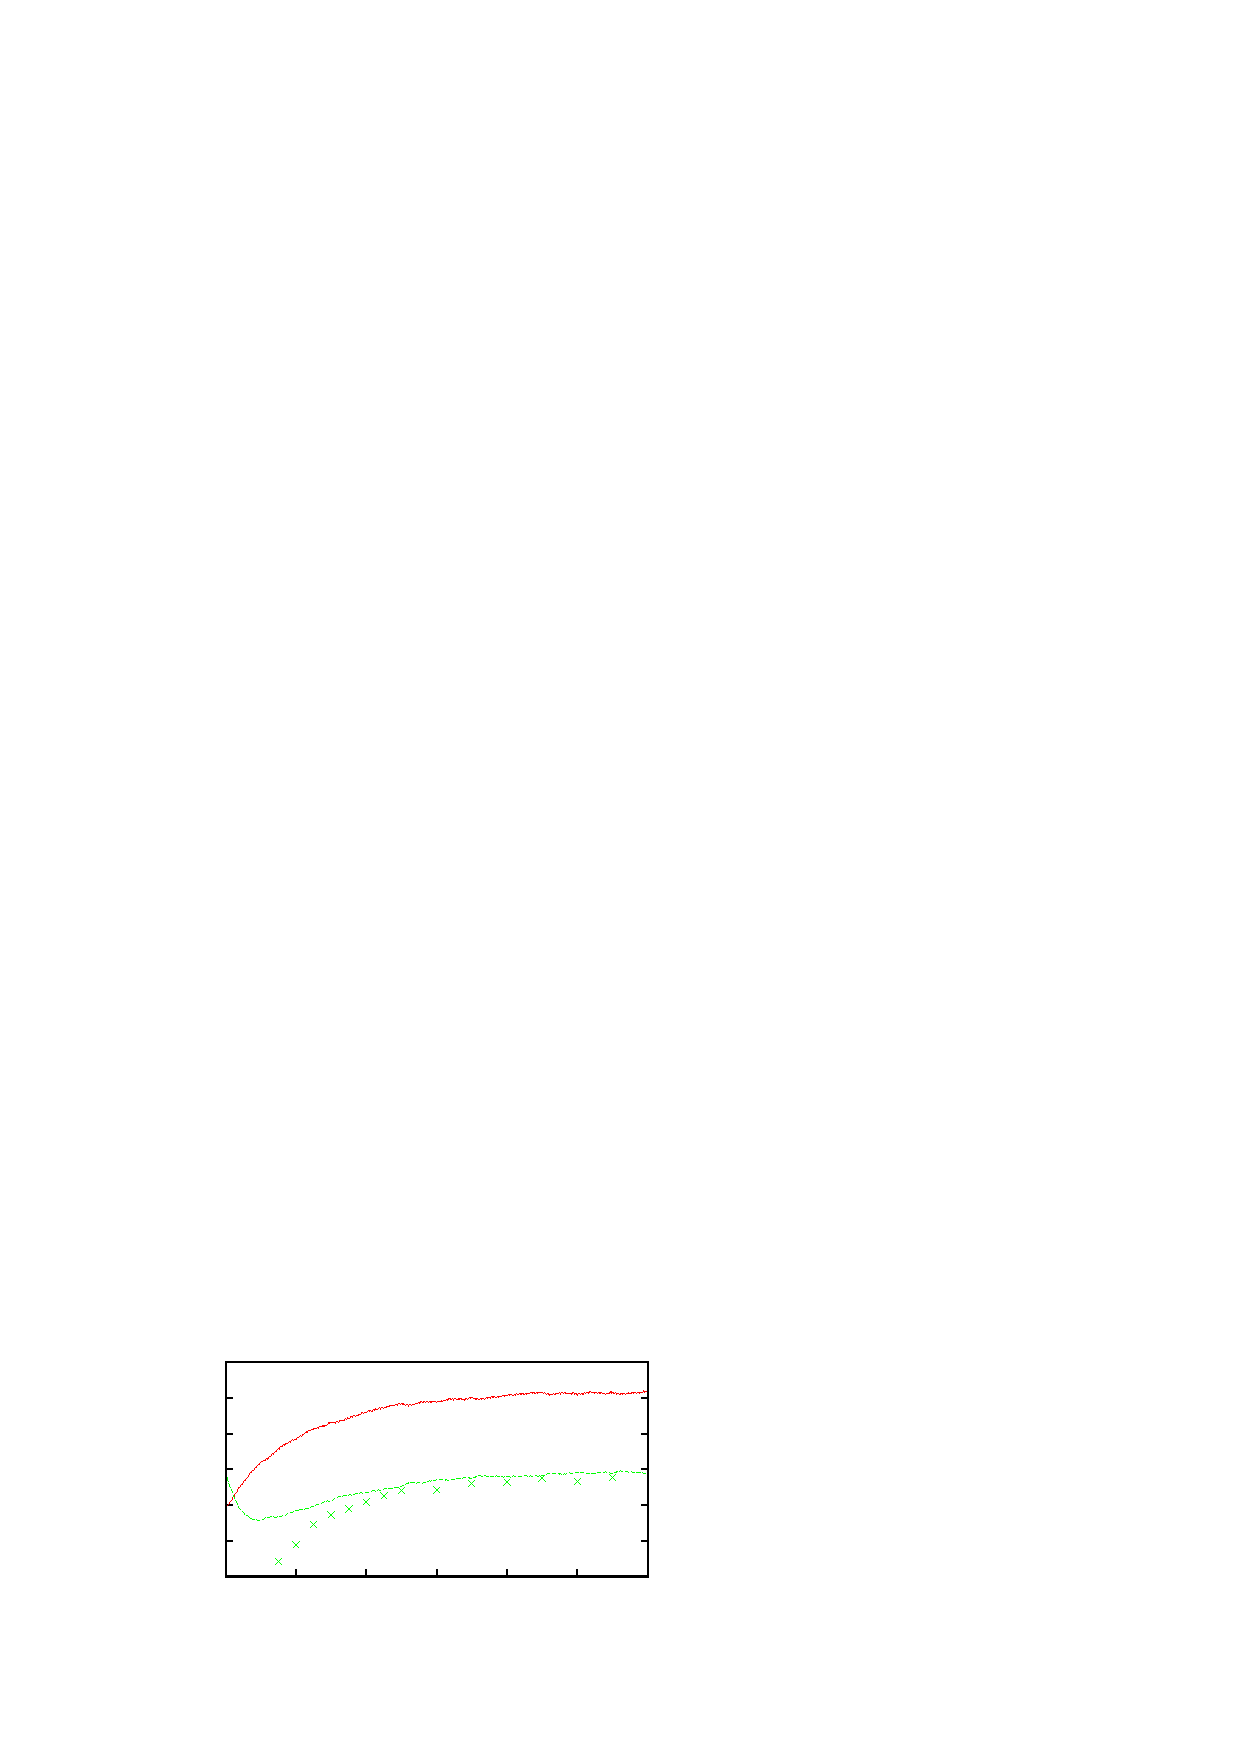
\includegraphics{realorgJB6}}%
    \gplfronttext
  \end{picture}%
\endgroup
 & \hspace{-2.1cm}%GNUPLOT: LaTeX picture with Postscript
\begin{picture}(0,0)%
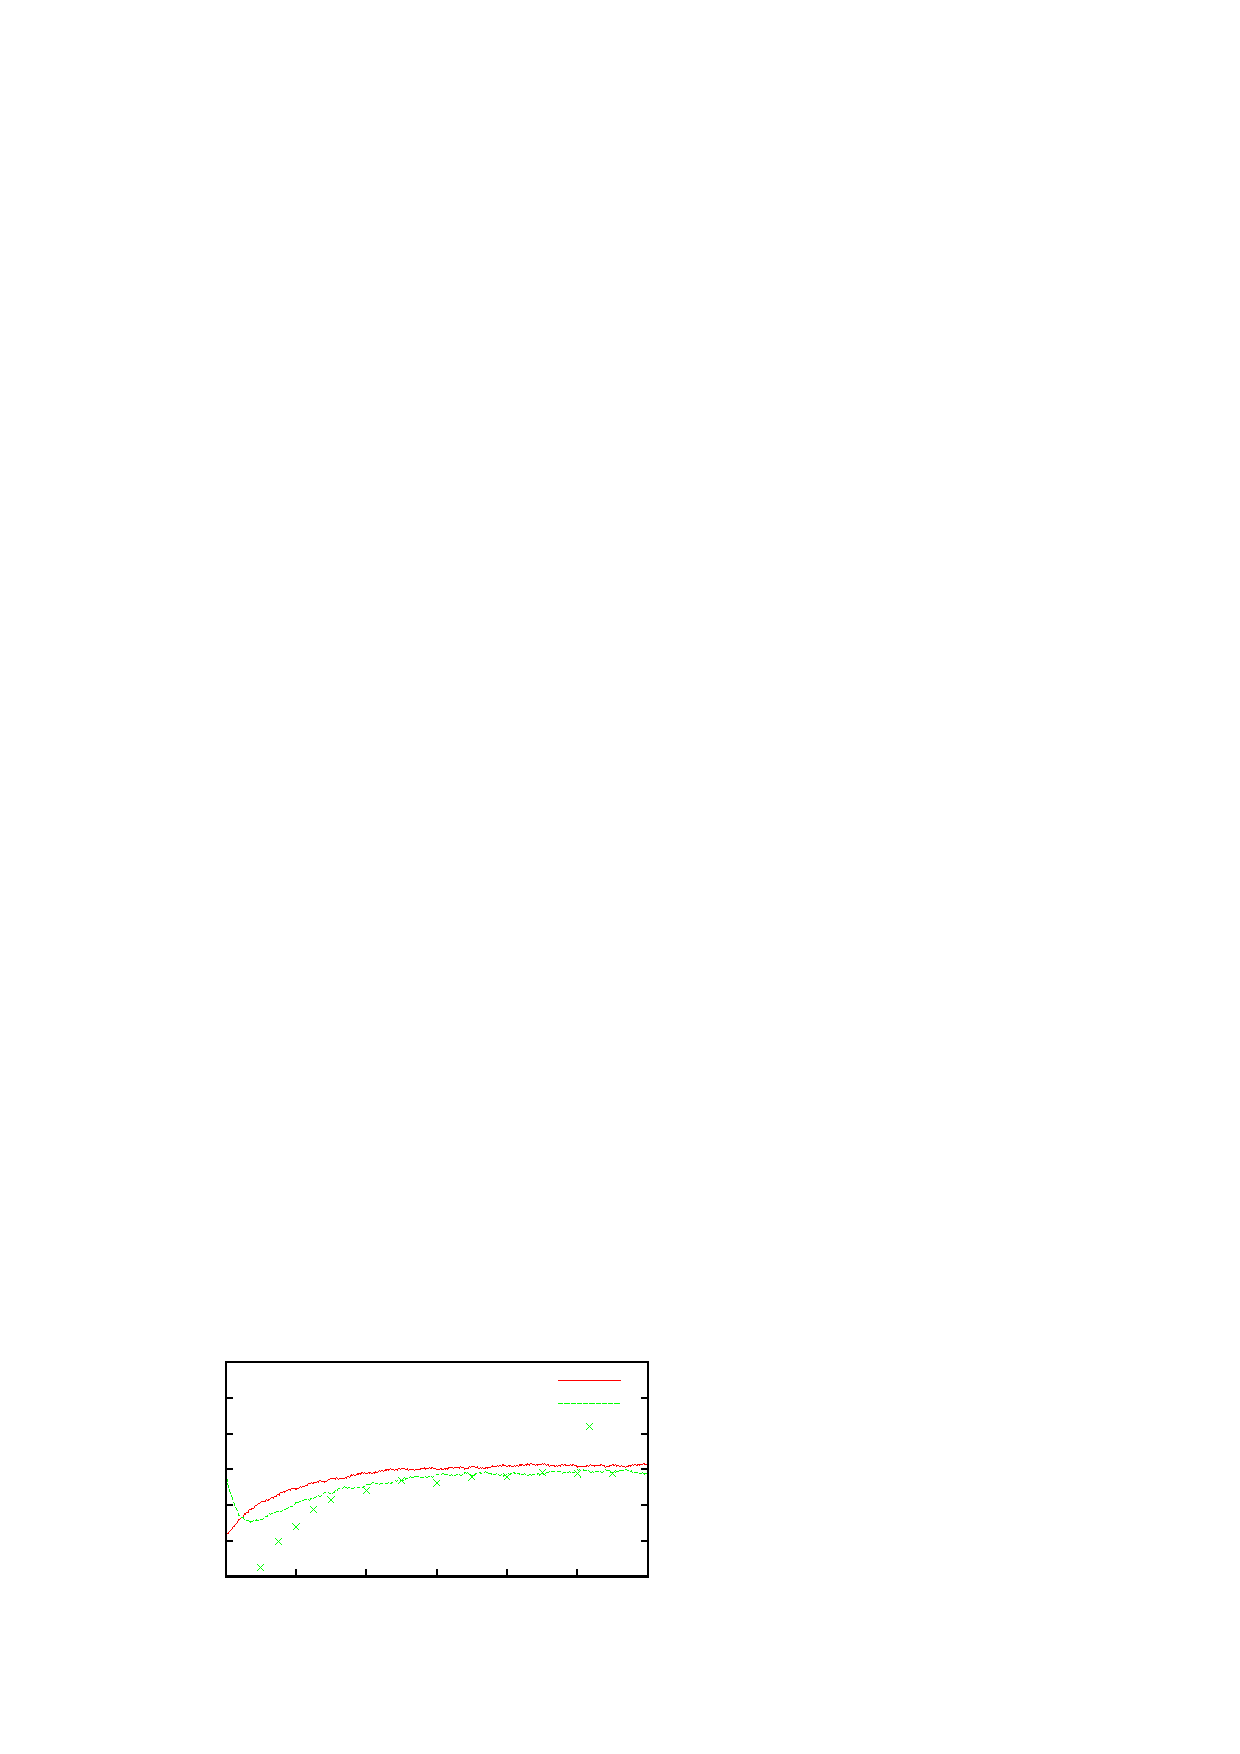
\includegraphics{realorgJB1}%
\end{picture}%
\begingroup
\setlength{\unitlength}{0.0200bp}%
\begin{picture}(18000,10800)(0,0)%
\put(2200,3300){\makebox(0,0)[r]{\strut{} 0}}%
\put(2200,4458){\makebox(0,0)[r]{\strut{} 0.2}}%
\put(2200,5617){\makebox(0,0)[r]{\strut{} 0.4}}%
\put(2200,6775){\makebox(0,0)[r]{\strut{} 0.6}}%
\put(2200,7933){\makebox(0,0)[r]{\strut{} 0.8}}%
\put(2200,9092){\makebox(0,0)[r]{\strut{} 1}}%
\put(2200,10250){\makebox(0,0)[r]{\strut{} 1.2}}%
\put(2475,2750){\makebox(0,0){\strut{}2000}}%
\put(3808,2750){\makebox(0,0){\strut{}2100}}%
\put(5140,2750){\makebox(0,0){\strut{}2200}}%
\put(6473,2750){\makebox(0,0){\strut{}2300}}%
\put(7805,2750){\makebox(0,0){\strut{}2400}}%
\put(9138,2750){\makebox(0,0){\strut{}2500}}%
\put(10470,2750){\makebox(0,0){\strut{}2600}}%
\put(11803,2750){\makebox(0,0){\strut{}2700}}%
\put(13135,2750){\makebox(0,0){\strut{}2800}}%
\put(14468,2750){\makebox(0,0){\strut{}2900}}%
\put(15800,2750){\makebox(0,0){\strut{}3000}}%
\put(16075,3300){\makebox(0,0)[l]{\strut{} 20}}%
\put(16075,4458){\makebox(0,0)[l]{\strut{} 30}}%
\put(16075,5617){\makebox(0,0)[l]{\strut{} 40}}%
\put(16075,6775){\makebox(0,0)[l]{\strut{} 50}}%
\put(16075,7933){\makebox(0,0)[l]{\strut{} 60}}%
\put(16075,9092){\makebox(0,0)[l]{\strut{} 70}}%
\put(16075,10250){\makebox(0,0)[l]{\strut{} 80}}%
\put(550,6775){\rotatebox{90}{\makebox(0,0){\strut{}Humus (\%)}}}%
\put(17449,6775){\rotatebox{90}{\makebox(0,0){\strut{}SOM1 (\%)}}}%
\put(9137,1925){\makebox(0,0){\strut{}Year}}%
\put(3687,825){\makebox(0,0)[l]{\strut{}Humus}}%
\put(3687,275){\makebox(0,0)[l]{\strut{}SOM1}}%
\put(12137,825){\makebox(0,0)[l]{\strut{}SOM1 quasi-equilibrium}}%
\end{picture}%
\endgroup
\endinput

  \end{tabular}
  \caption{Long term simulation on a sand (left column) and sandy loam
    soil (right column) of total organic matter (\textsc{tom}) in
    percent of soil dry bulk mass (fully drawn line, left axes) and
    \textsc{som1} in percent of of total \textsc{som} (dotted line,
    right axes) with management changing from: (top row) high to low C
    input and (bottom row) low to high C input.  The $\times$'s
    indicate the initialization of \textsc{som1} for the current
    amount of \textsc{tom} estimated by the quasi-equilibrium.}
  \label{fig:long}
\end{figure*}
A more moderate change is depicted in Fig.~\ref{fig:orgJB1}.
\begin{figure}[htbp]
  \begin{tabular}{l}
    \% of soil\hfill{}Sandy loam, medium input\hfill{}\% of SOM\hspace{1cm} \\
    \hspace{-1.5cm}% GNUPLOT: LaTeX picture with Postscript
\begingroup
  \makeatletter
  \providecommand\color[2][]{%
    \GenericError{(gnuplot) \space\space\space\@spaces}{%
      Package color not loaded in conjunction with
      terminal option `colourtext'%
    }{See the gnuplot documentation for explanation.%
    }{Either use 'blacktext' in gnuplot or load the package
      color.sty in LaTeX.}%
    \renewcommand\color[2][]{}%
  }%
  \providecommand\includegraphics[2][]{%
    \GenericError{(gnuplot) \space\space\space\@spaces}{%
      Package graphicx or graphics not loaded%
    }{See the gnuplot documentation for explanation.%
    }{The gnuplot epslatex terminal needs graphicx.sty or graphics.sty.}%
    \renewcommand\includegraphics[2][]{}%
  }%
  \providecommand\rotatebox[2]{#2}%
  \@ifundefined{ifGPcolor}{%
    \newif\ifGPcolor
    \GPcolorfalse
  }{}%
  \@ifundefined{ifGPblacktext}{%
    \newif\ifGPblacktext
    \GPblacktexttrue
  }{}%
  % define a \g@addto@macro without @ in the name:
  \let\gplgaddtomacro\g@addto@macro
  % define empty templates for all commands taking text:
  \gdef\gplbacktext{}%
  \gdef\gplfronttext{}%
  \makeatother
  \ifGPblacktext
    % no textcolor at all
    \def\colorrgb#1{}%
    \def\colorgray#1{}%
  \else
    % gray or color?
    \ifGPcolor
      \def\colorrgb#1{\color[rgb]{#1}}%
      \def\colorgray#1{\color[gray]{#1}}%
      \expandafter\def\csname LTw\endcsname{\color{white}}%
      \expandafter\def\csname LTb\endcsname{\color{black}}%
      \expandafter\def\csname LTa\endcsname{\color{black}}%
      \expandafter\def\csname LT0\endcsname{\color[rgb]{1,0,0}}%
      \expandafter\def\csname LT1\endcsname{\color[rgb]{0,1,0}}%
      \expandafter\def\csname LT2\endcsname{\color[rgb]{0,0,1}}%
      \expandafter\def\csname LT3\endcsname{\color[rgb]{1,0,1}}%
      \expandafter\def\csname LT4\endcsname{\color[rgb]{0,1,1}}%
      \expandafter\def\csname LT5\endcsname{\color[rgb]{1,1,0}}%
      \expandafter\def\csname LT6\endcsname{\color[rgb]{0,0,0}}%
      \expandafter\def\csname LT7\endcsname{\color[rgb]{1,0.3,0}}%
      \expandafter\def\csname LT8\endcsname{\color[rgb]{0.5,0.5,0.5}}%
    \else
      % gray
      \def\colorrgb#1{\color{black}}%
      \def\colorgray#1{\color[gray]{#1}}%
      \expandafter\def\csname LTw\endcsname{\color{white}}%
      \expandafter\def\csname LTb\endcsname{\color{black}}%
      \expandafter\def\csname LTa\endcsname{\color{black}}%
      \expandafter\def\csname LT0\endcsname{\color{black}}%
      \expandafter\def\csname LT1\endcsname{\color{black}}%
      \expandafter\def\csname LT2\endcsname{\color{black}}%
      \expandafter\def\csname LT3\endcsname{\color{black}}%
      \expandafter\def\csname LT4\endcsname{\color{black}}%
      \expandafter\def\csname LT5\endcsname{\color{black}}%
      \expandafter\def\csname LT6\endcsname{\color{black}}%
      \expandafter\def\csname LT7\endcsname{\color{black}}%
      \expandafter\def\csname LT8\endcsname{\color{black}}%
    \fi
  \fi
  \setlength{\unitlength}{0.0500bp}%
  \begin{picture}(6120.00,3024.00)%
    \gplgaddtomacro\gplbacktext{%
      \csname LTb\endcsname%
      \put(1034,440){\makebox(0,0)[r]{\strut{} 0}}%
      \put(1034,827){\makebox(0,0)[r]{\strut{} 0.2}}%
      \put(1034,1213){\makebox(0,0)[r]{\strut{} 0.4}}%
      \put(1034,1600){\makebox(0,0)[r]{\strut{} 0.6}}%
      \put(1034,1987){\makebox(0,0)[r]{\strut{} 0.8}}%
      \put(1034,2373){\makebox(0,0)[r]{\strut{} 1}}%
      \put(1034,2760){\makebox(0,0)[r]{\strut{} 1.2}}%
      \put(1166,220){\makebox(0,0){\strut{}2000}}%
      \put(1841,220){\makebox(0,0){\strut{}2100}}%
      \put(2517,220){\makebox(0,0){\strut{}2200}}%
      \put(3192,220){\makebox(0,0){\strut{}2300}}%
      \put(3867,220){\makebox(0,0){\strut{}2400}}%
      \put(4543,220){\makebox(0,0){\strut{}2500}}%
      \put(5218,220){\makebox(0,0){\strut{}2600}}%
      \put(5350,440){\makebox(0,0)[l]{\strut{} 20}}%
      \put(5350,827){\makebox(0,0)[l]{\strut{} 30}}%
      \put(5350,1213){\makebox(0,0)[l]{\strut{} 40}}%
      \put(5350,1600){\makebox(0,0)[l]{\strut{} 50}}%
      \put(5350,1987){\makebox(0,0)[l]{\strut{} 60}}%
      \put(5350,2373){\makebox(0,0)[l]{\strut{} 70}}%
      \put(5350,2760){\makebox(0,0)[l]{\strut{} 80}}%
    }%
    \gplgaddtomacro\gplfronttext{%
    }%
    \gplbacktext
    \put(0,0){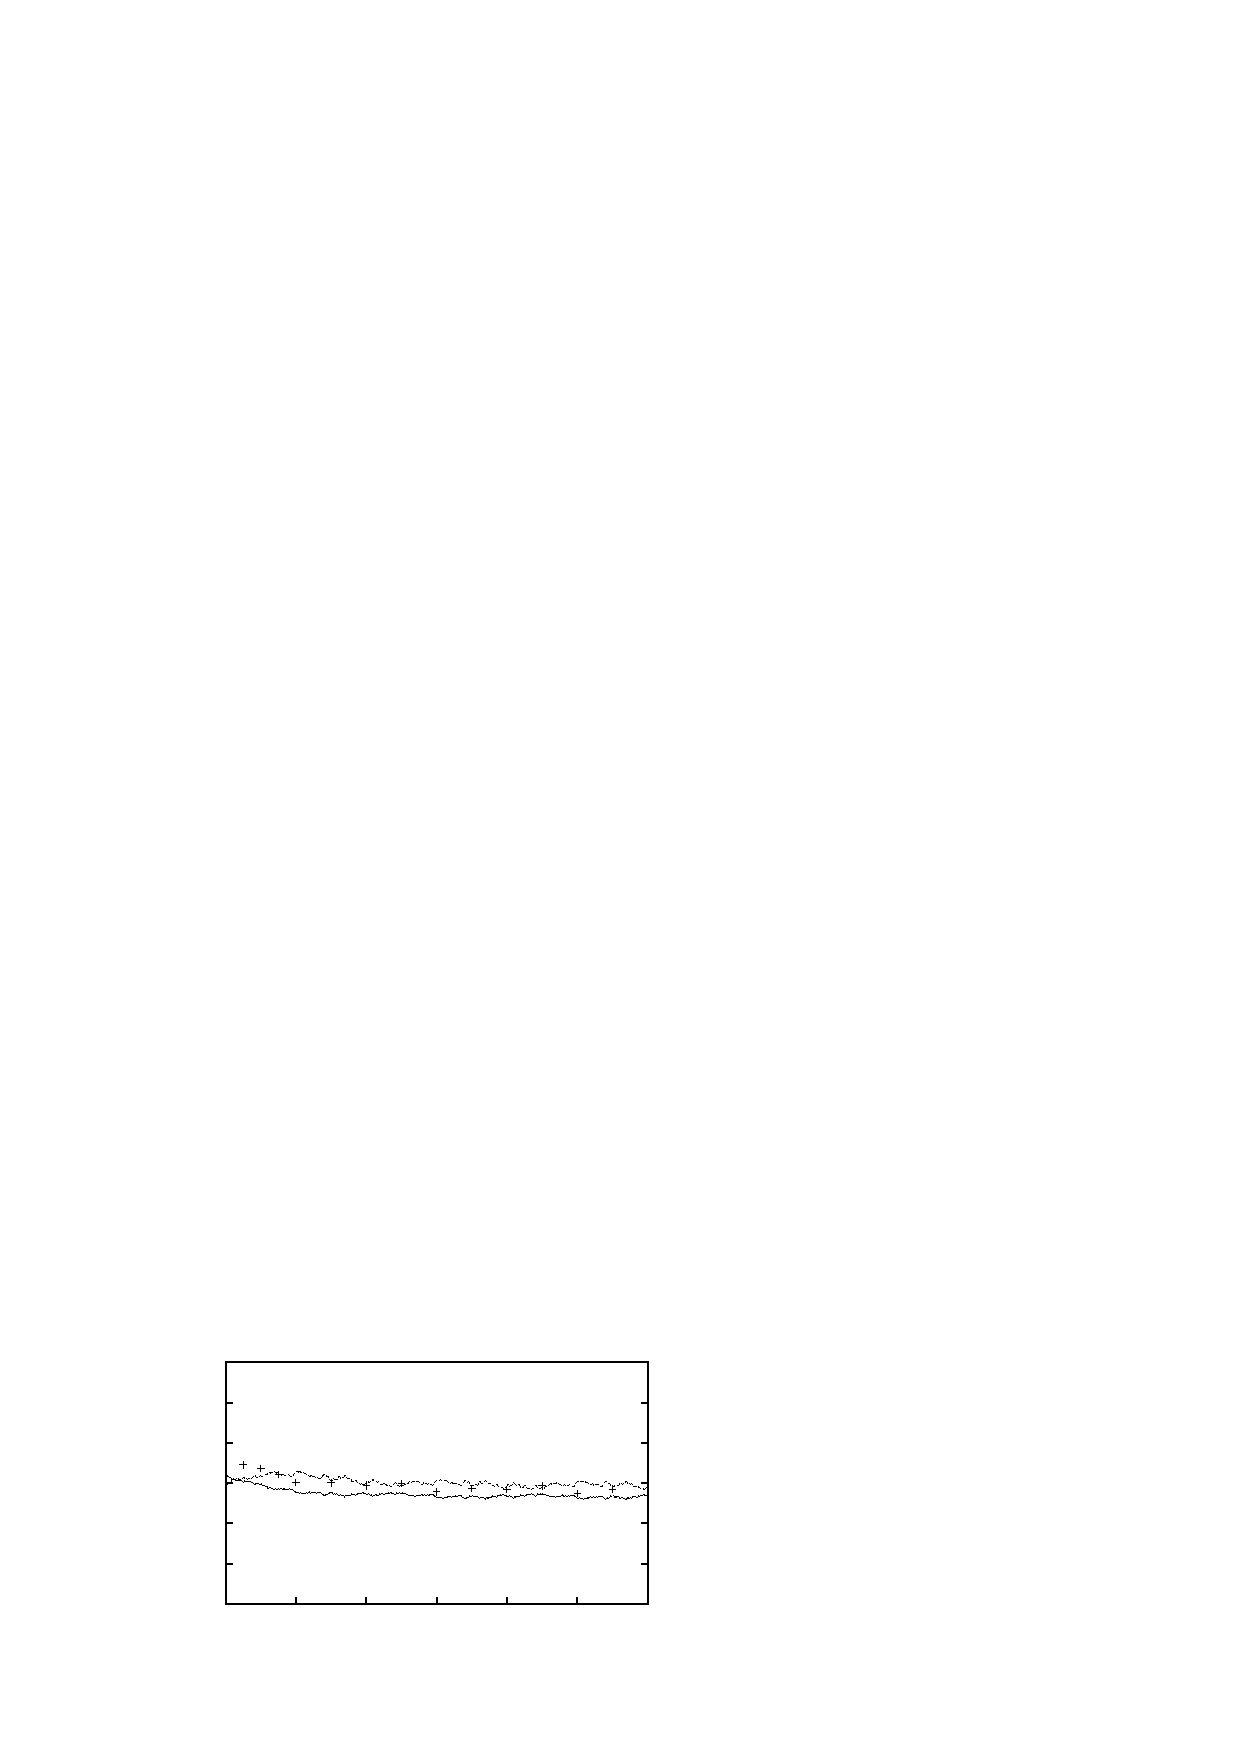
\includegraphics{realmediumJB1}}%
    \gplfronttext
  \end{picture}%
\endgroup

  \end{tabular}
  \caption{Long term simulation on a sand of total organic matter
    (\textsc{tom}) in percent of dry bulk mass (left axis) and
    \textsc{som1} in percent of toal \textsc{som} (right axis) with
    management changing from high to medium C input. Simulated values
    are on the dotted line. The $\times$'s indicate the initialization
    of \textsc{som1} for the current humus level estimated by the
    proposed quasi-equilibrium.}
  \label{fig:orgJB1}
\end{figure}

After a decrease in input (Fig.~\ref{fig:long}, top), the organic
content of the soil decreases, but the easily degradable \textsc{som}
pool (\textsc{som2}) decreases faster than the more resistant pool
(\textsc{som1}), so the relative \textsc{som1} fraction increases
temporarily.  A similar effect can be seen after an increase of input
(Fig.~\ref{fig:long}, bottom), where the easily degradable
\textsc{som} pool build up faster than the resistant pool, and
relative \textsc{som1} fraction decreases temporarily while the total
organic matter builds up.

Equilibrium is reached after 200 (sandy loam, increasing input) to 600
(sand, decreasing input) years.  Since the longest experimental trial
used for validating the organic matter model in Daisy is 70 years
\citep{smith97-compar}, these results must all be viewed as
extrapolation.  Equilibrium is reached sooner for the sandy loam than
for the sand, and sooner for increasing input than for decreasing
input.  For decreasing input, quasi-equilibrium is reached after 150
years (on sand) or 100 years (on sandy loam), well before equilibrium.
For increasing input, quasi-equilibrium is reached at approximately
the same time as equilibrium.

The initialization method developed here is easy to understand and use
by the user. The two mandatory numbers are the total content of
organic matter, and an estimate of how much carbon has been added to
the system per year in the recent decades. The total content of
organic matter is directly measurable and the carbon input estimated
by the user, for example from the use of Daisy simulations. None of
the these numbers need to be changed when the model itself is changed.

As can be seen, the time to reach a new equilibrium after a large
change in farming practice can be several centuries, which makes it
safe to assume that Danish farming land is not in equilibrium. At such
a time scale, not only farming practice but also climate is going to
change. 

After lowering carbon input, we reach quasi-equilibirum at around a
third of the time we use to reach full equilinbrium.  For a large
change, this unfortunetely is not practically useful, as even for the
scenario where the quasi-equilibirum does best (the sandy loam), it
still takes a century to reach quasi-equilibirum.  In the case of
raising carbon input, quasi-equilibirum doesn't seem to be approached
faster than full equilinbrium.  For relatively small changes in carbon
input, either method works fine.

In all scenarios, the quasi-equilibirum estimate for \textsc{som1}
approaches the value predicted for full equilibrium (49\%,
\citet{daisy-init}) as the dynamic model itself approaches
equilibrium.  Since the quasi-equilibirum estimate is strongly
dependent on abiotic factors, this indicates that, despite the
non-linearity of the abiotic effect functions, using the average value
work well, under the conditions examined.  The average value can be
found with a Daisy simulation.

Despite the increased clay content, which should slow down turnover in
the system, the sandy loam reach both quasi-equilibirum and full
equilibrium faster than the sand, because of the increased humidity of
the soil during the summer.  Which indicate that both initialization
assumptions would result in estimates of the \textsc{som} partitining
that are closer to the dynamic model, under climate where organic
matter turnover is faster due to heat or humidity.

Another possible aspect for further study would be other organic
matter model parametrizations, especially parametrizations where
difference in the turnover rate between the \textsc{som} pools is
higher.

\conclusions

The quasi-equilibirum assumption doesn't work under Danish conditions
with the current organic matter model in Daisy.

\addcontentsline{toc}{section}{\numberline{}References}
\bibliography{../daisy}

\end{document}

%%% Local Variables:
%%% mode: latex
%%% TeX-master: t
%%% End:
